\documentclass[a4paper, 14pt]{extarticle}%тип документа
\date{}

\usepackage{indentfirst}


\usepackage{graphicx}
\usepackage{cmap}
\usepackage[T2A]{fontenc}
\usepackage[utf8]{inputenc}

%%%Библиотеки
	%\usepackage[warn]{mathtext}	
	\usepackage[T2A]{fontenc} % кодировка
	\usepackage[utf8]{inputenc} % кодировка исходного текста
	\usepackage[english,russian]{babel} % локализация и переносы
	\usepackage{caption}
	\usepackage{listings}
	\usepackage{amsmath,amsfonts,amssymb,amsthm,mathtools}
	\usepackage{wasysym}
	\usepackage{graphicx}%Вставка картинок правильная
	\usepackage{float}%"Плавающие" картинки
	\usepackage{wrapfig}%Обтекание фигур (таблиц, картинок и прочего)
	\usepackage{fancyhdr} %загрузим пакет
	\usepackage{lscape}
	\usepackage{xcolor}
	\usepackage[normalem]{ulem}
	\usepackage{hyperref}

%%%Конец библиотек

%%\renewcommand{\footrulewidth}{ .0em }
\usepackage[english,russian]{babel}
\usepackage{multirow} % Слияние строк в таблице
\newcommand
{\un}[1]
{\ensuremath{\text{#1}}}


%Русский язык
\usepackage[T2A]{fontenc} %кодировка
\usepackage[utf8]{inputenc} %кодировка исходного кода
\usepackage[english,russian]{babel} %локализация и переносы

%Таблицы
%Математика
\usepackage{amsmath, amsfonts, amssymb, amsthm, mathtools}

%отступы 
\usepackage[left=2cm,right=2cm,top=2cm,bottom=3cm,bindingoffset=0cm]{geometry}

%Вставка картинок
\usepackage{graphicx}
\usepackage{wrapfig, caption}
\graphicspath{}
\DeclareGraphicsExtensions{.pdf,.png,.jpg, .jpeg}
\newcommand\ECaption[1]{%
     \captionsetup{font=footnotesize}%
     \caption{#1}}


%Графики
\usepackage{pgfplots}
\pgfplotsset{compat=1.9}
\usepackage[english,russian]{babel}
\usepackage{multirow} % Слияние строк в таблице

%%%Настройка ссылок
	\hypersetup
	{
		colorlinks=true,
		linkcolor=blue,
		filecolor=magenta,
		urlcolor=blue
	}
%%%Конец настройки ссылок


%%%Настройка колонтитулы
	\pagestyle{fancy}
	\fancyhead{}
	\fancyhead[L]{Лабораторная работа}
	\fancyhead[R]{Талашкевич Даниил, группа Б01-009}
	\fancyfoot[C]{\thepage}
%%%конец настройки колонтитулы\


\begin{document}


%%%Начало титульника
\begin{titlepage}

	\newpage
	\begin{center}
		\normalsize Московский физико-технический институт \\(госудраственный 			университет)
	\end{center}

	\vspace{6em}

	\begin{center}
		\Large Лабораторная работа по РТ цепям\\
	\end{center}

	\vspace{1em}

	\begin{center}
		\large \textbf{Связанные колебательные контуры [20]}
	\end{center}

	\vspace{2em}

	\begin{center}
		\large Талашкевич Даниил Александрович\\
		Группа Б01-009
	\end{center}

	\vspace{\fill}

	\begin{center}
	Долгопрудный \\2021
	\end{center}
	
\end{titlepage}
%%%Конец Титульника

%%%Настройка оглавления и нумерации страниц
	\thispagestyle{empty}
	\newpage
	\tableofcontents
	\newpage
	\setcounter{page}{1}
%%%Настройка оглавления и нумерации страниц


\section{Задание №1. Система с индуктивной связью.}

\subsection{Знакомство с составом подготовленных графиков}

Откроем подготовленную модель и смотрим на полученные графики для режима $AC$:

\begin{figure}[h!]
	\centering
			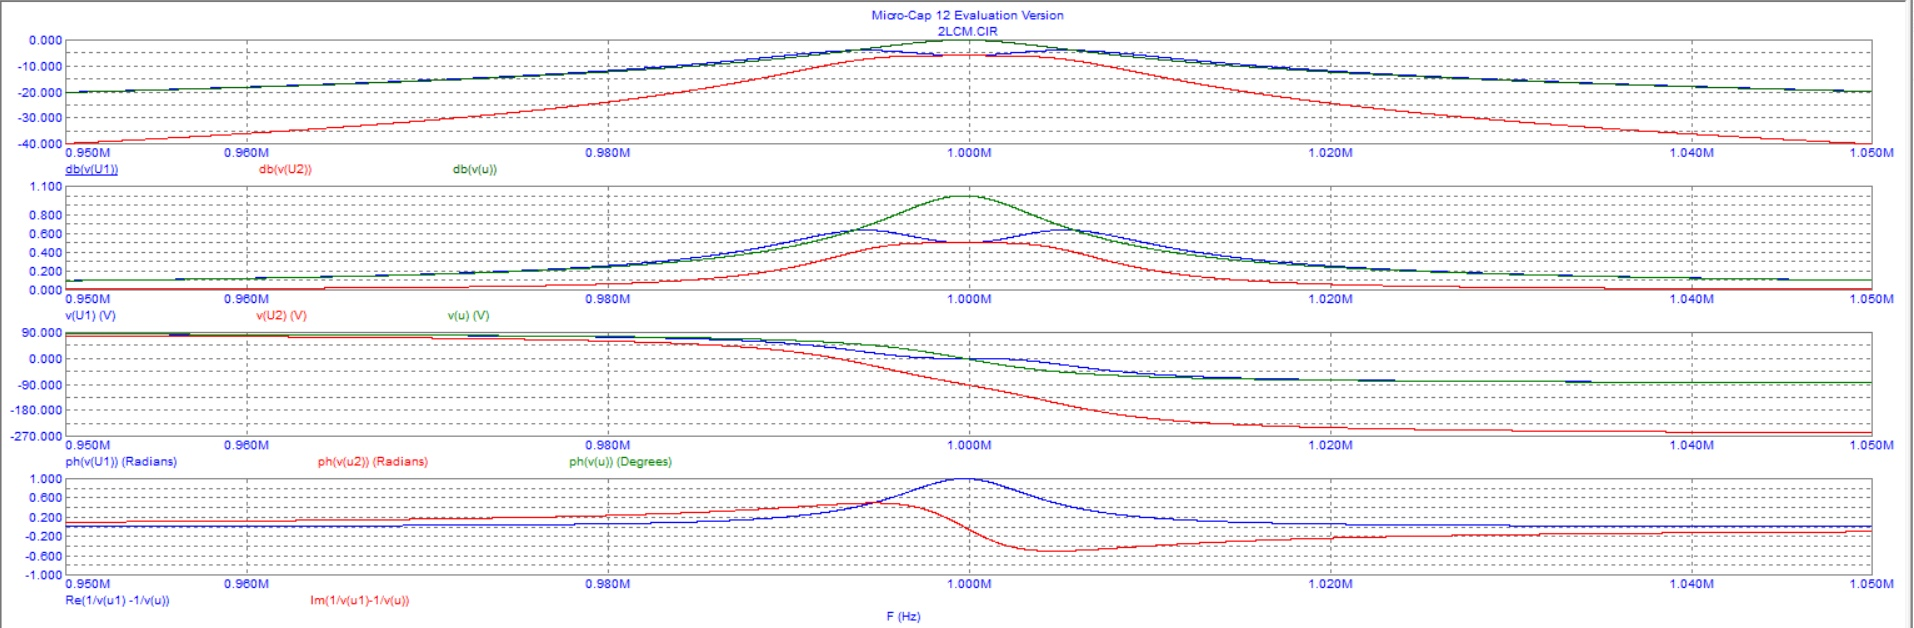
\includegraphics[width=1.1\linewidth]{1.1.jpg}
			%\caption{Задание 1, пункт 1}
	\label{A}
\end{figure}

Здесь $\textbf{плот 1}$ -- частотные характеристики для $u, u_1, u_2$ в децибелах, $\textbf{плот 2}$ -- частотные характеристики, $\textbf{плот 3}$ -- фазовые характеристики, $\textbf{плот 4}$ -- мнимая и вещественная часть вносимой проводимости.


\subsection{плот 2 (частотная характеристика)}

Оставляем плот 2 графиков частотных характеристик и при критической связи изучим их поведение при варьировании параметров контуров.
\newline
Варьируем параметры контуров:
\newline
$R_{1(2)} = [100k,  \: 900k \:| \: 200k]$ и емкости первого и второго контуров следующим образом $C_{1(2)} [159.2p, \: 165p \: | \: 1p]$, $C_{1(2)} [159.2p, \: 165p \: | \: -1p]$

\begin{figure}[h!]
	\centering
			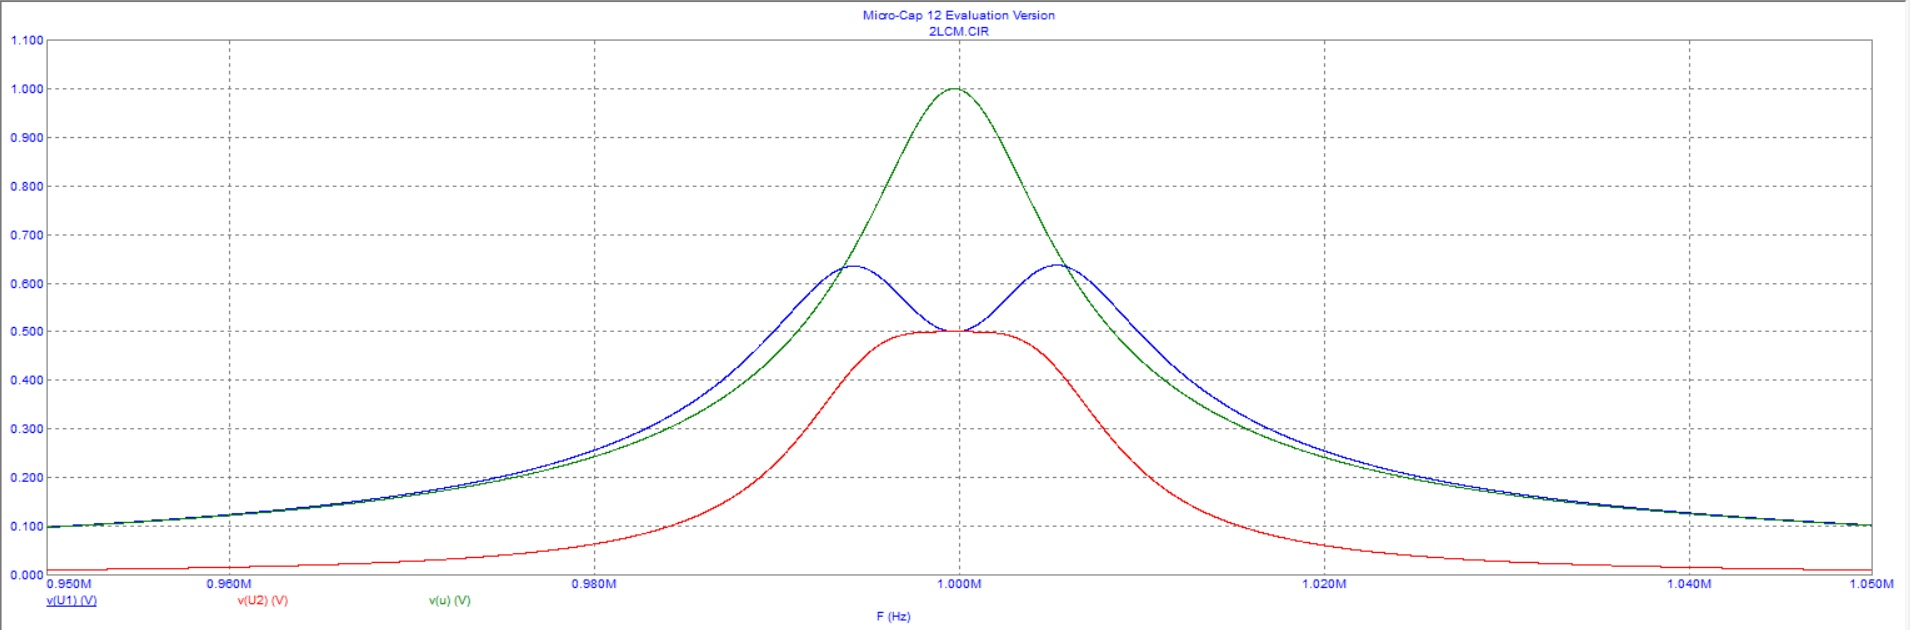
\includegraphics[width=1.1\linewidth]{1.2.jpg}
            %\caption{Задание 1, пункт 2}
	\label{A}
\end{figure}

\begin{figure}[h!]
	\centering
			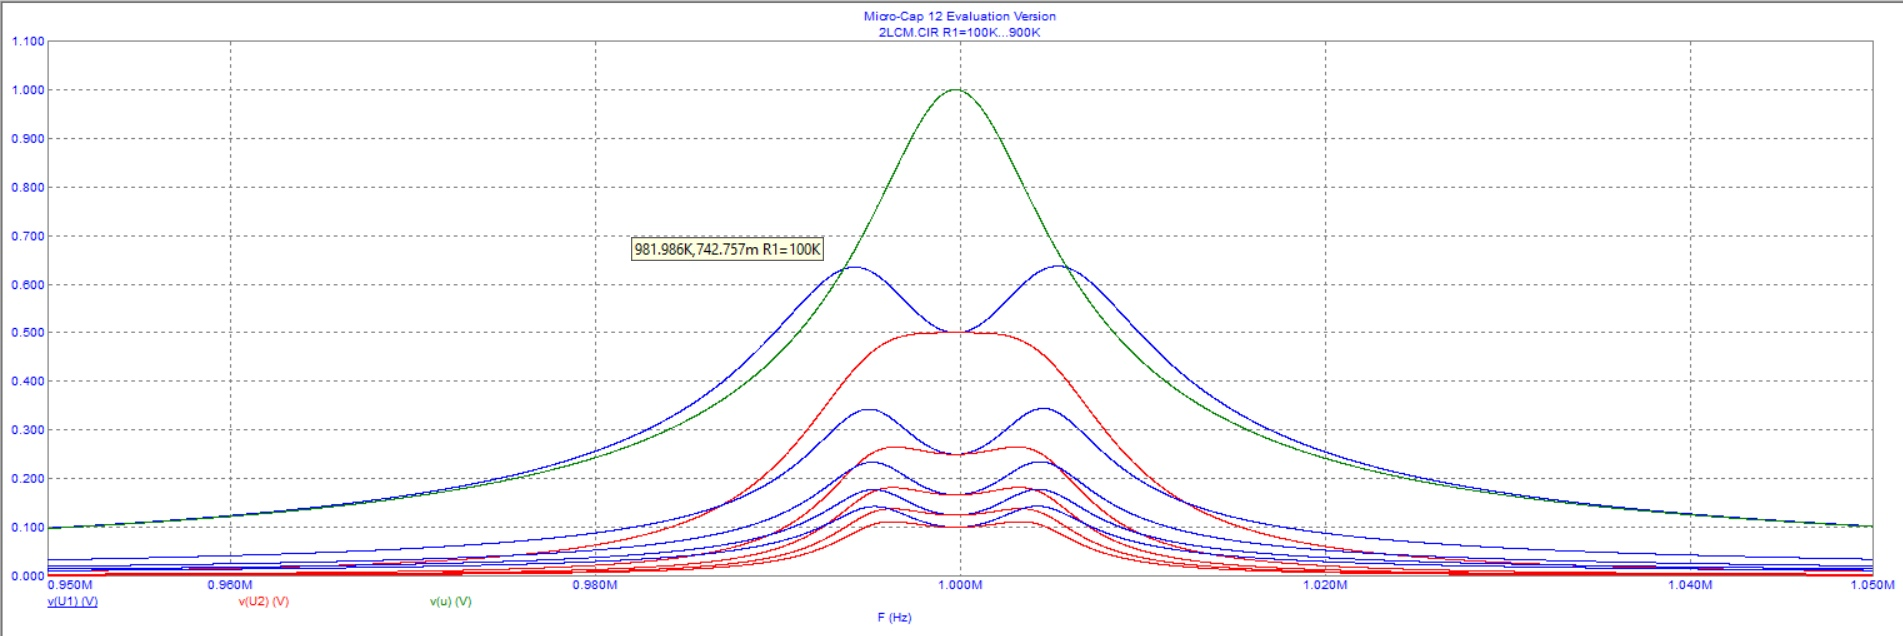
\includegraphics[width=1.1\linewidth]{1.2_varR1.jpg}
            \caption{варьирование $R_1$}
	\label{A}
\end{figure}

\begin{figure}[h!]
	\centering
			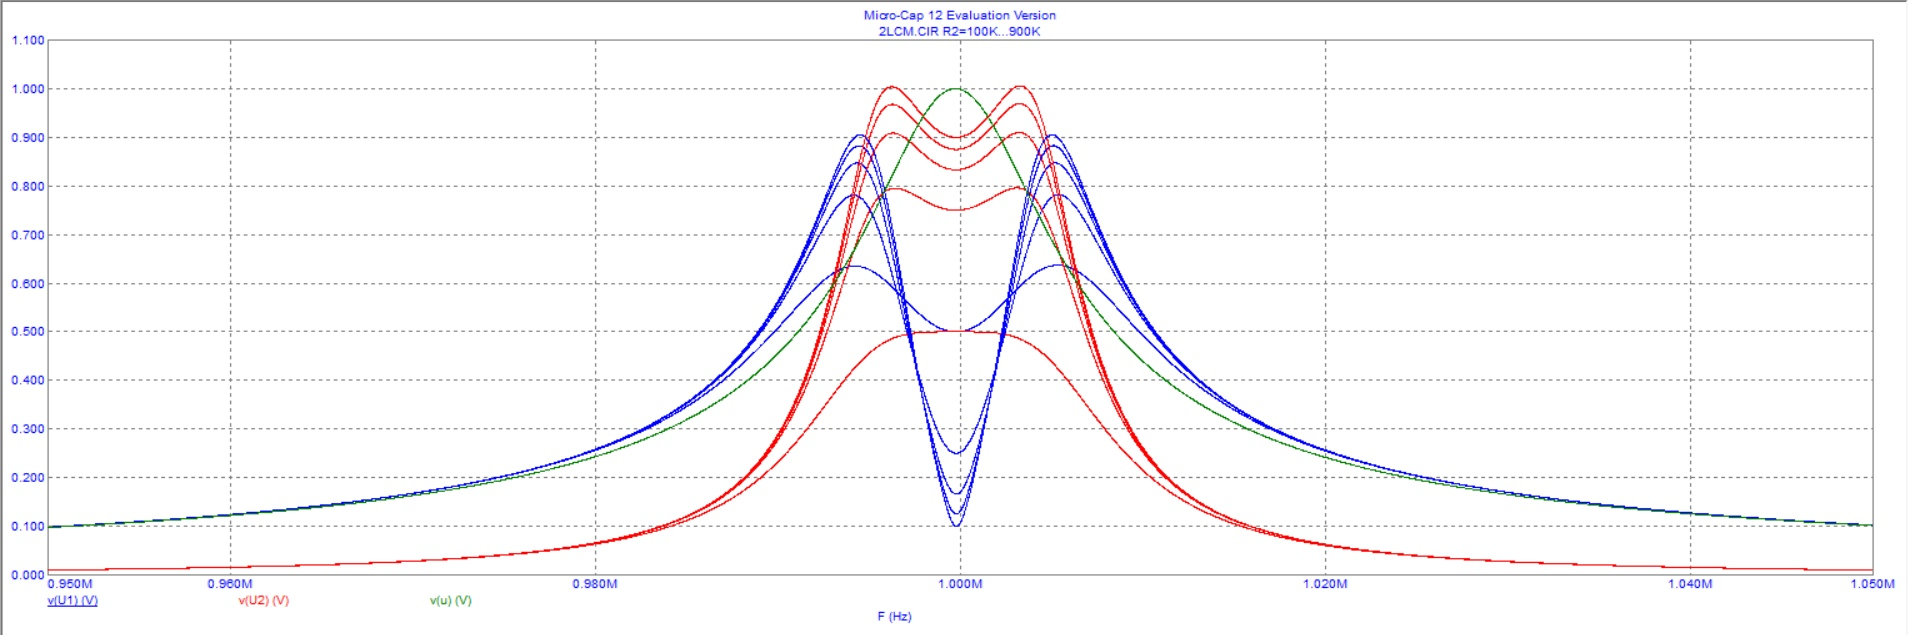
\includegraphics[width=1.1\linewidth]{1.2_varR2.jpg}
            \caption{варьирование $R_2$}
	\label{A}
\end{figure}


\begin{figure}[h!]
	\centering
			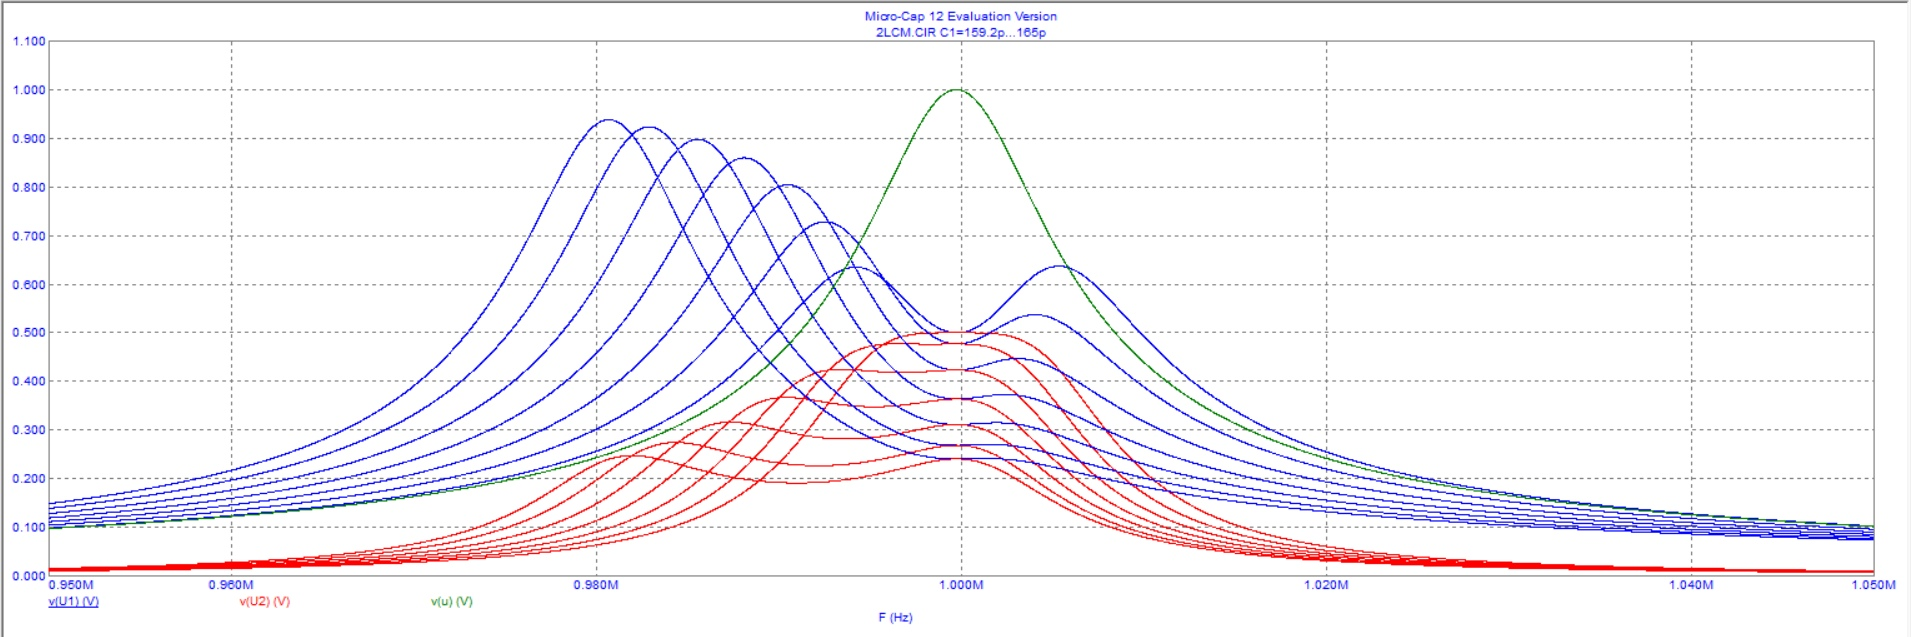
\includegraphics[width=1.1\linewidth]{1.2_varC1.jpg}
            \caption{варьирование $C_1 [159.2p, 165p|1p]$}
	\label{A}
\end{figure}


\begin{figure}[h!]
	\centering
			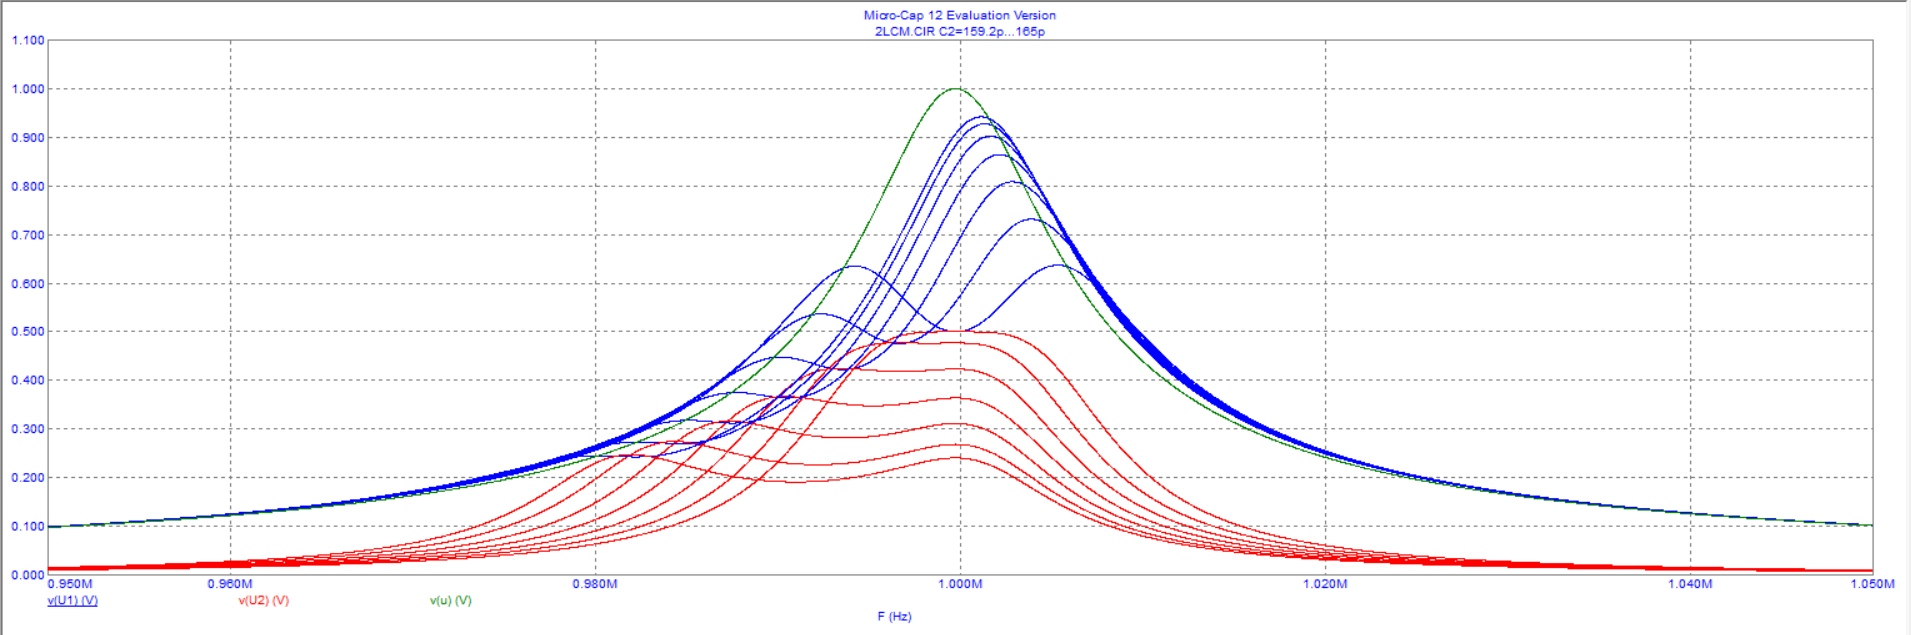
\includegraphics[width=1.1\linewidth]{1.2_varC2.jpg}
            \caption{варьирование $C_2 [159.2p, 165p|1p]$}
	\label{A}
\end{figure}

\newpage

\subsection{плот 3 (изучение фазовых характеристик)}

Изучим поведение резонансных кривых и фазовых характеристик при следующем варьировании $F = [0.2, 1|0.2]$ и $F = [1, 5|1]$. Как результат измерений, проверим формулы

\[ u_1(f_0) = \frac{1}{1+F^2},\ u_2(f_0) = \frac{F}{1 + F^2} \]

и измерим границы диапазонов изменения фаз на первом и втором контурах.

\begin{figure}[h!]
	\centering
			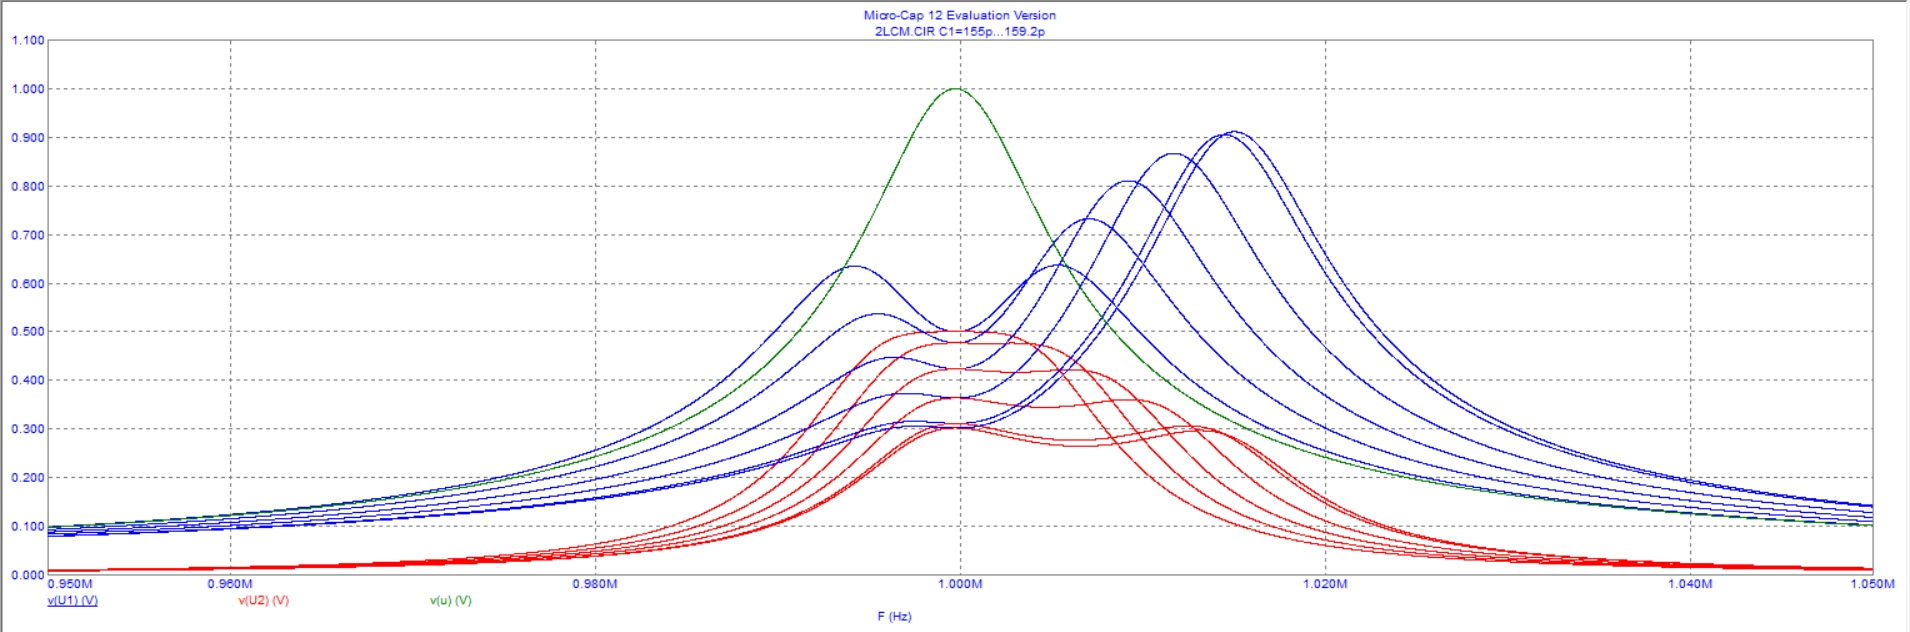
\includegraphics[width=1.1\linewidth]{1.2_varC1_3.jpg}
            \caption{варьирование $C_1 [159.2p,155p|-1p]$}
	\label{A}
\end{figure}

\begin{figure}[h!]
	\centering
			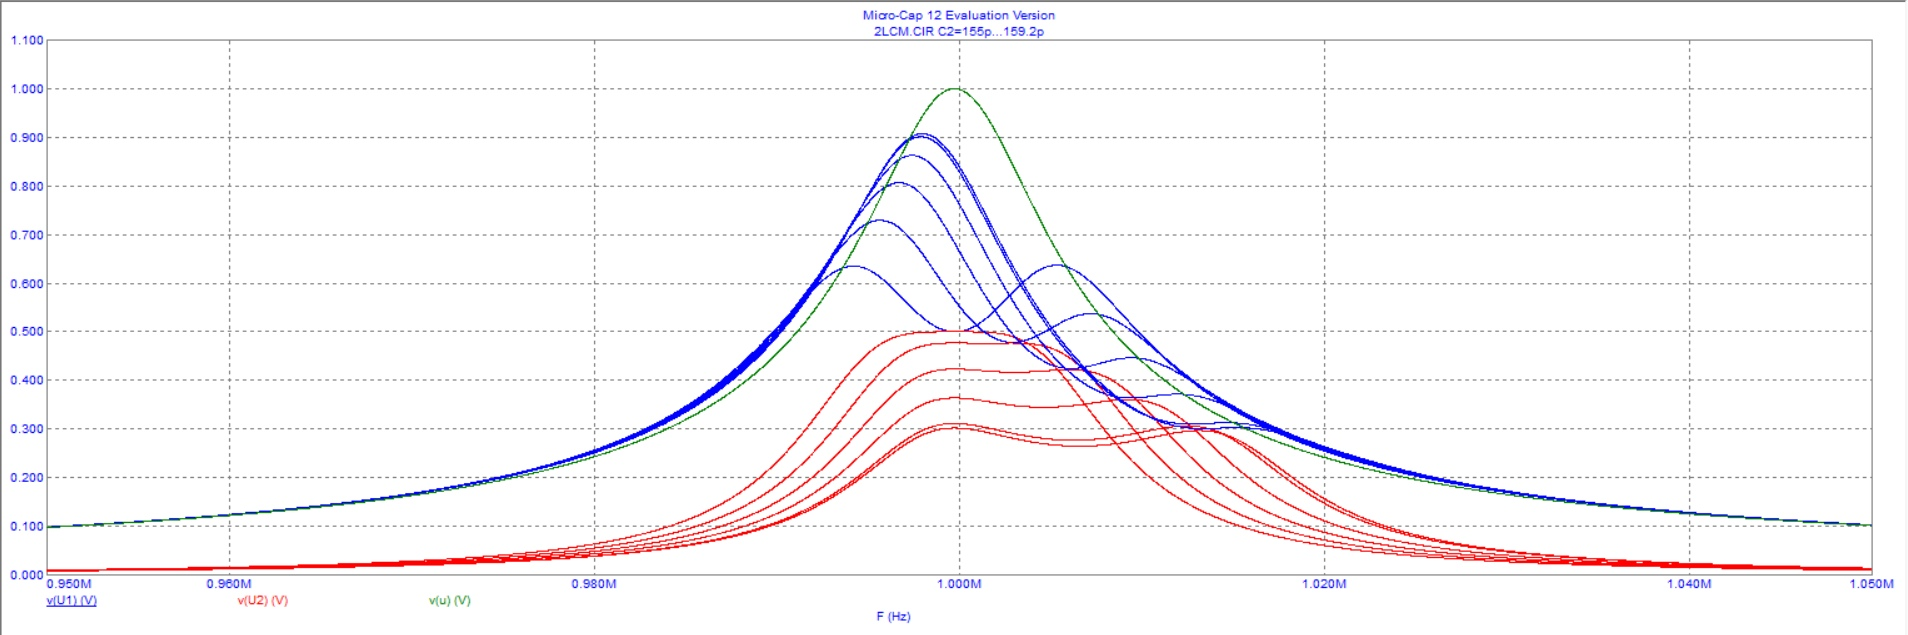
\includegraphics[width=1.1\linewidth]{1.2_varC1_4.jpg}
            \caption{варьирование $C_2 [159.2p,155p|-1p]$}
	\label{A}
\end{figure}

\begin{figure}[h!]
	\centering
			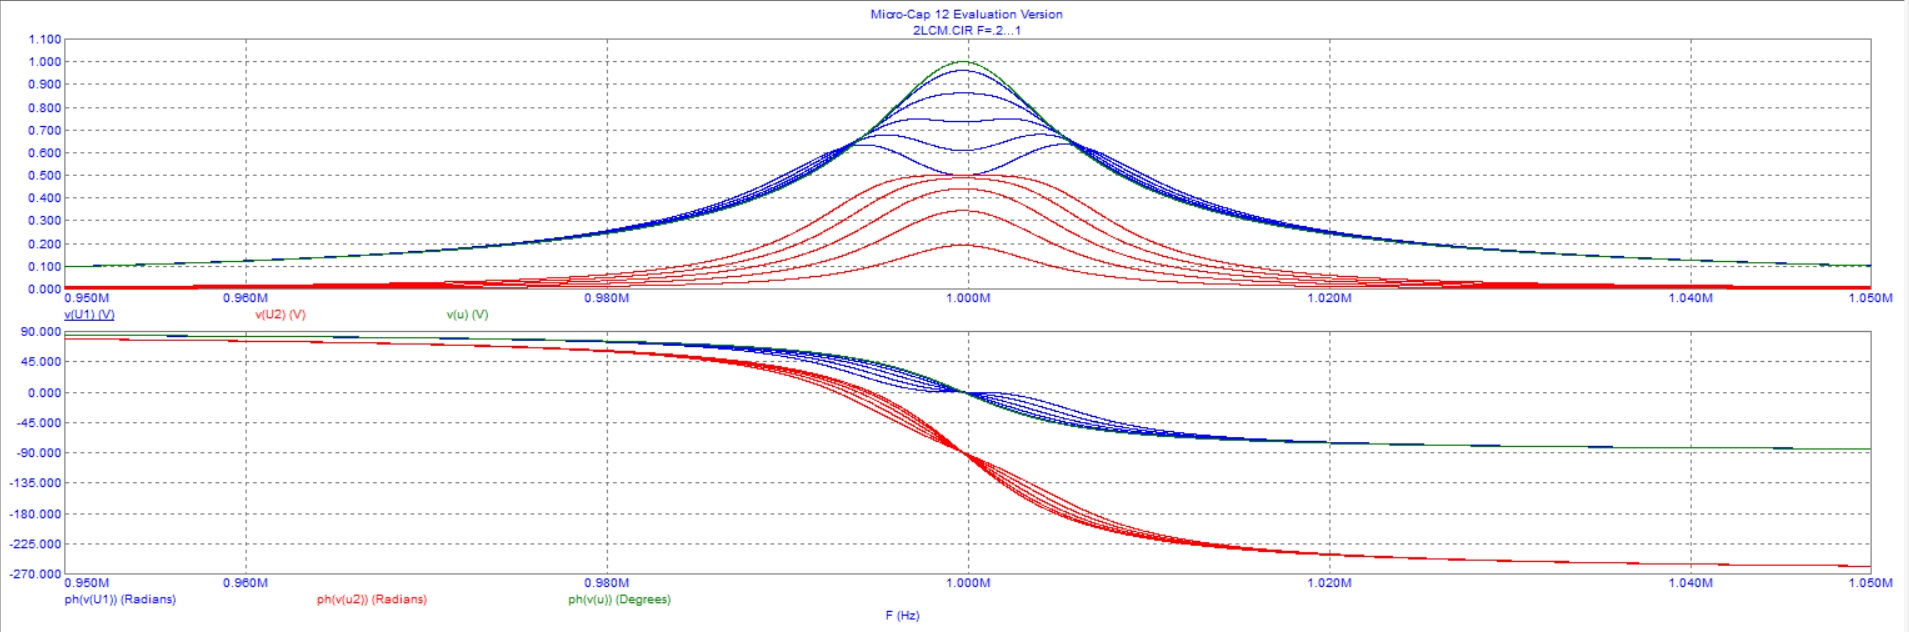
\includegraphics[width=1.1\linewidth]{1.2varF1.jpg}
            \caption{варьирование $F [0.2, 1|0.2]$}
	\label{A}
\end{figure}


\begin{figure}[h!]
	\centering
			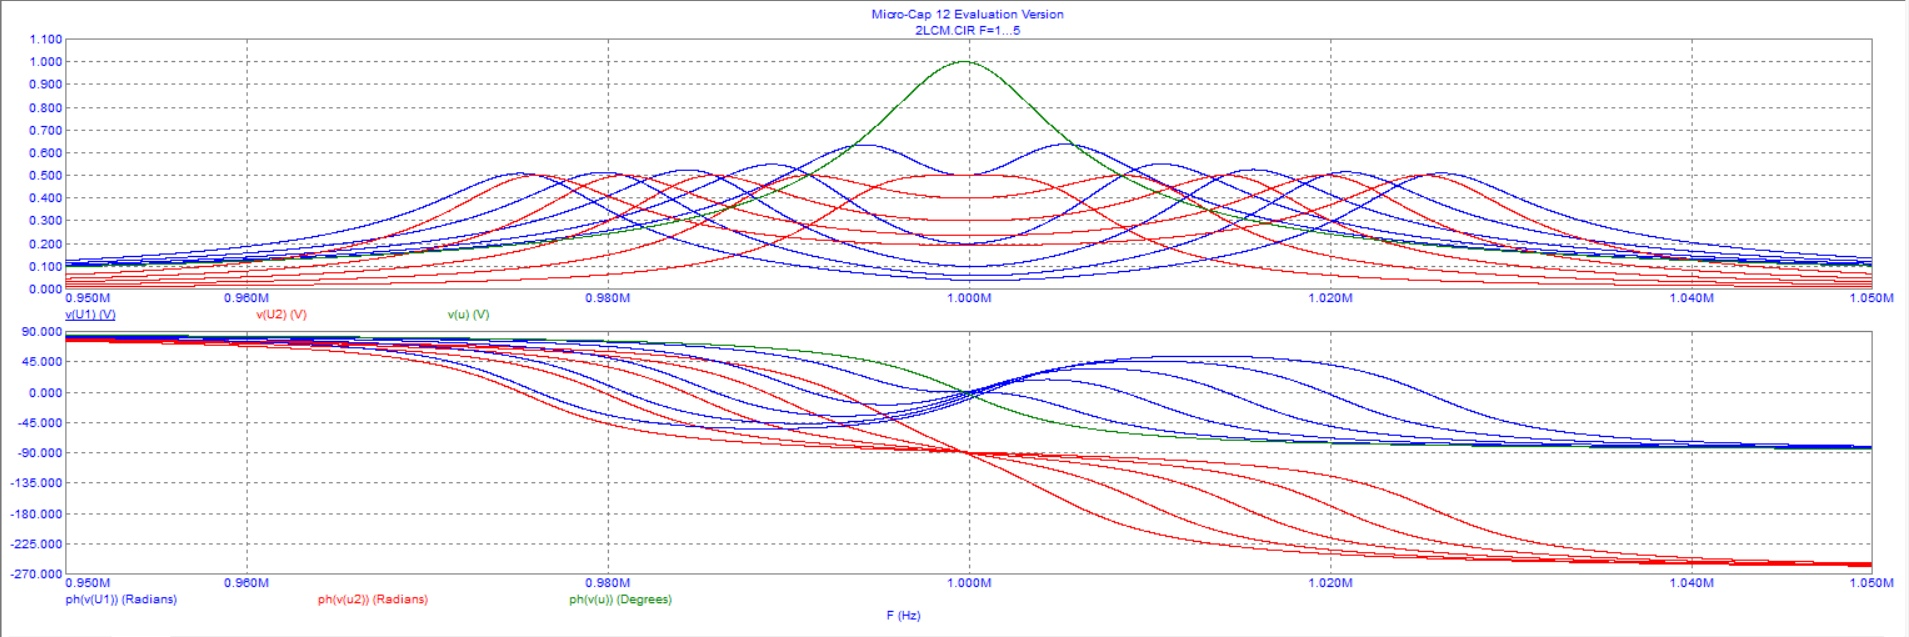
\includegraphics[width=1.1\linewidth]{1.2varF2.jpg}
            \caption{варьирование $F [0.2, 1|0.2]$}
	\label{A}
\end{figure}

\newpage

на первом контуре -- от $-77.010^{\circ}$ до $75.155^{\circ}$, на втором контуре -- от $-238.454^{\circ}$ до $60.139^{\circ}$. В свою очередь разность фаз между напряжениями на контурах на частоте $f_0$: $93.711^{\circ}$.

Измерив уровни $u_1(f_0)$, $u_2(f_0)$ при различных $F$, чтобы проверить формулы.
 

\begin{table}[h]
	\centering
	\begin{tabular}{|c|c|c|c|}
		\hline
		$F$                         & $1$ & $0.5$ & $2$ \\ \hline
		$u_1(f_0)_{\text{эксп}}$          & 0.5 & 0.8   & 0.2 \\ \hline
		$u_1(f_0)_{\text{теор}}$ & 0.5 & 0.8   & 0.2 \\ \hline \hline
		$u_2(f_0)_{\text{эксп}}$          & 0.5 & 0.4   & 0.2 \\ \hline
		$u_2(f_0)_{\text{теор}}$ & 0.5 & 0.4   & 0.2 \\ \hline
	\end{tabular}
	\caption{Проверка формул}
\end{table}

Из полученных значений можно сделать вывод, что формулы выполняются.


\subsection{провал и подъем}

В этом пункте измерим значения $F$, при которых возникает: 1) провал на первом контуре, b) провал на втором контуре c) подъём на фазовой характеристике первого контура.

Измерив частоты пересечения нуля фазовой характеристикой $u_1$ при $F = 5;10$, проверим приближённые ($f_0\pm FF_0$) и уточнённые ($f_0\sqrt{1\pm\frac{F}{Q}}$) формулы для частот полюсов.

Полученные значения:

a) 0.6
b) 1.1
c) 1.1

Частоты пересечения нуля ФХ $u_1$, при:

$F = 5: \nu = 976.120k, 1M, 1.025M$.

$F = 10: \nu = 953.43k, 1.005M, 1.054M$. 

\subsection{плот 1 (измерение ширины полосы)}

При критической связи измерим ширину полосы по уровню -3dB эталонного контура ($\Delta f = 10.273k$) и ширину полосы по уровню -9dB резонансной кривой на втором контуре ($\Delta f = 14.279k$). Убедимся, что их отношение составляет $\sqrt{2}$.


\begin{figure}[h!]
	\centering
			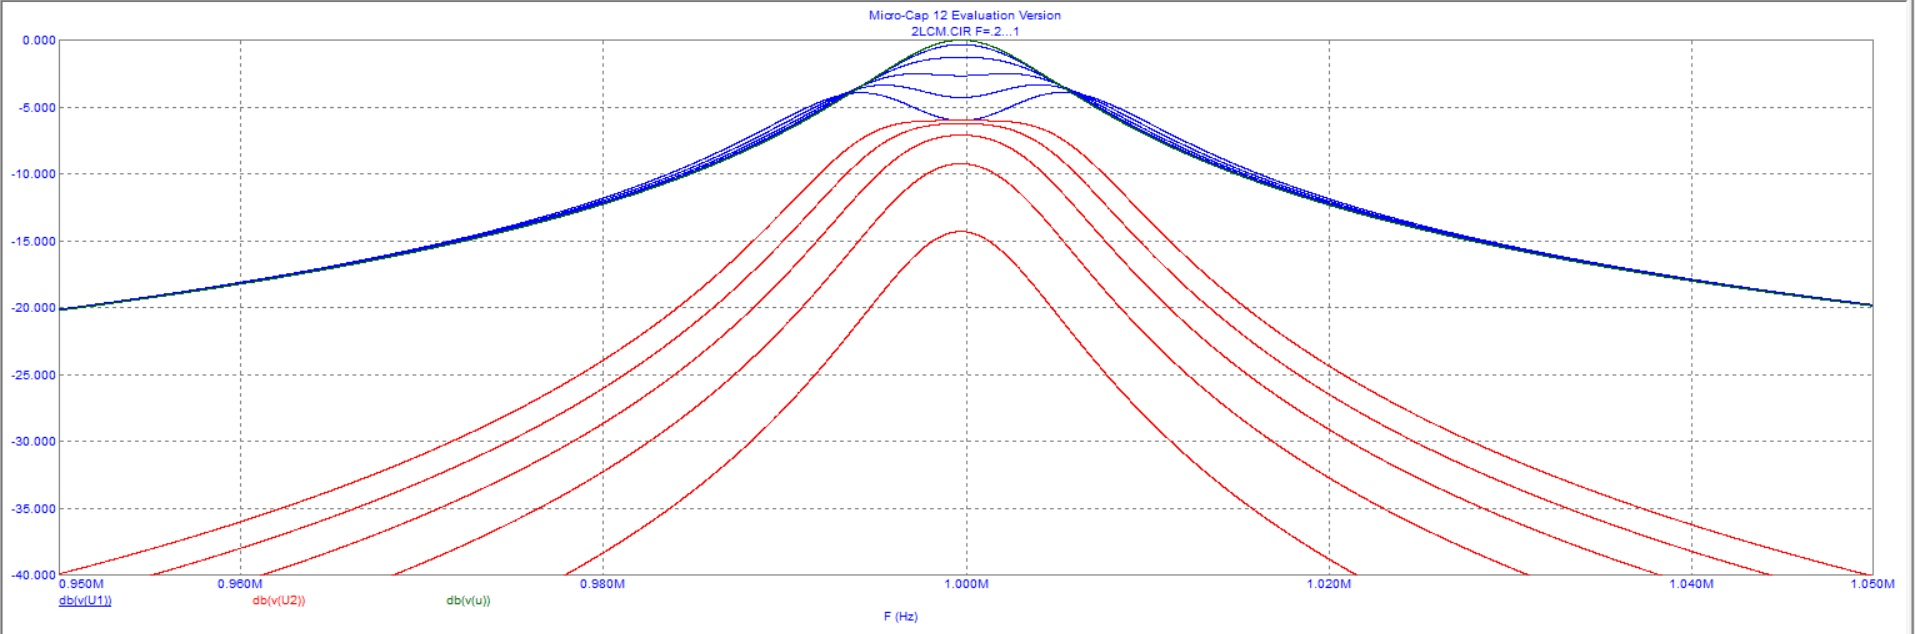
\includegraphics[width=1.1\linewidth]{1.5.jpg}
            %\caption{Задание 1,  пункт 5}
	\label{A}
\end{figure}

\begin{figure}[h!]
	\centering
			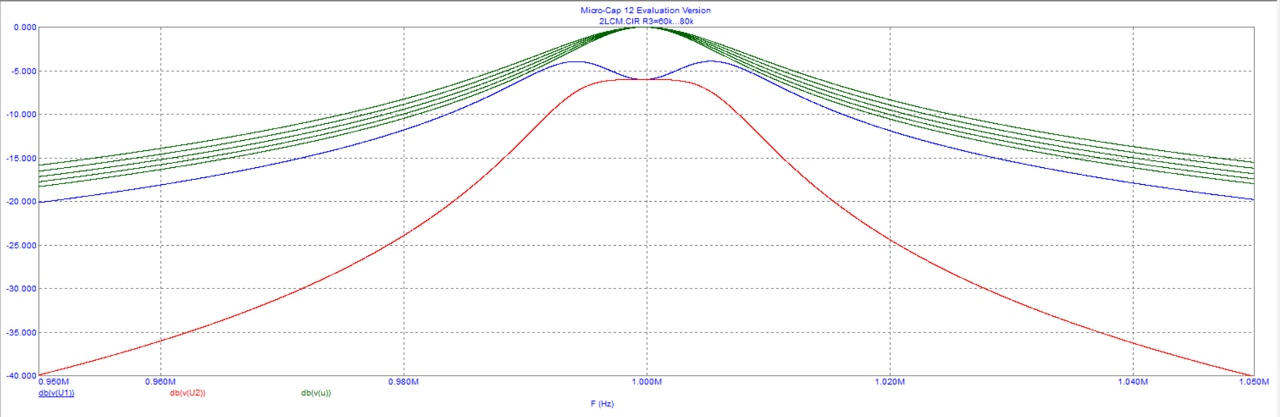
\includegraphics[width=1.1\linewidth]{1.5varR1.jpg}
            \caption{варьирование $R_3 [60k, 80k|5k]$}
	\label{A}
\end{figure}


Измерим уровни затухания критической кривой при сдвигах по частоте на декаду $F_0$, то есть на $\pm 10F_0 = \pm 50k$ (затухание -- $-34\frac{dB}{\text{дек}_{F_0}}$). Варьируя сопротивление потерь эталонного контура $R = [60k,~80k|5k]$, выясним, что при добротности $Q = 68.6$ ($R = 70k,~\Delta f = 14.557k$) его полоса сравнивается с полосой двухконтурной системы. Измерим затухание, вносимое эталонным контуром с этой добротностью при расстройках на декаду $F_0$ (затухание -- $-16.7\frac{dB}{\text{дека}_{F_0}}$). Оценим выигрыш двухконтурной системы по затуханию: выигрыш $\simeq~\text{2 раза}$.

~

\subsection{резонансные кривые}

Изучим поведение резонансных кривых при $F = [0.5,~1|0.1]$. Найдём значение $F = [0.65,~0.75|0.05]$, при котором полоса двухконтурной системы по критическому уровню -9dB сравнивается с полосой $10k$ эталонного контура: $F = 0.75$. При этом значении $F$ оценим выигрыш по затуханию при расстройке на декаду $F_0$ двухконтурной системы по сравнению с эталоном: у эталона -- $-19.75\frac{dB}{\text{дек}_{F_0}}$, у двухконтурной системы -- $-36.45\frac{dB}{\text{дек}_{F_0}} \Longrightarrow \text{выигрыш $\simeq$ 2 раза}$.

\begin{figure}[h!]
	\centering
			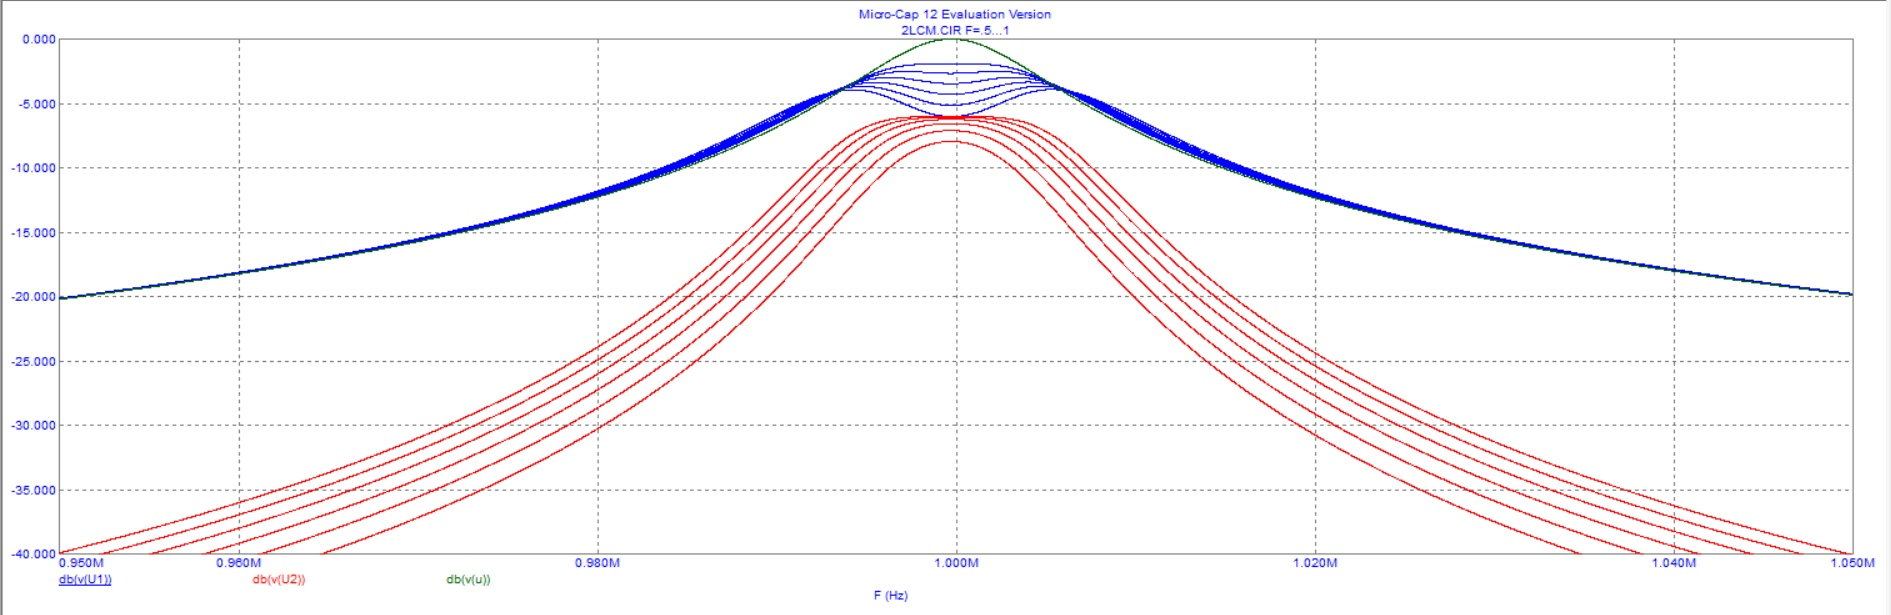
\includegraphics[width=1.1\linewidth]{1.6varF1.jpg}
            \caption{варьирование $F [0.5, 1|0.1]$}
	\label{A}
\end{figure}

\begin{figure}[h!]
	\centering
			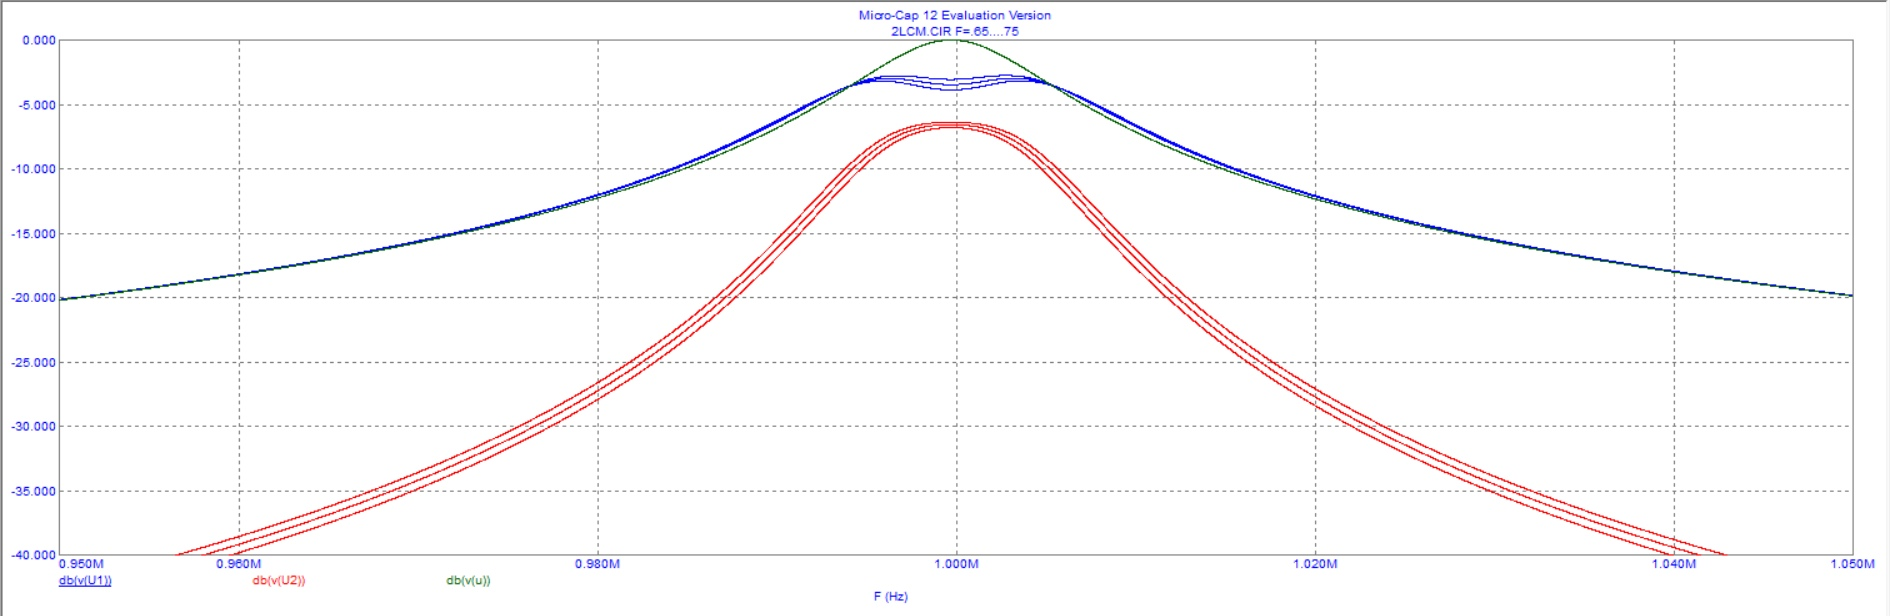
\includegraphics[width=1.1\linewidth]{1.6varF2.jpg}
            \caption{варьирование $F [0.65, 0.75|0.05]$}
	\label{A}
\end{figure}

~

\subsection{резонансные кривые}

Измерим значение $F$ из диапазона $F = [2.2,~2.6|0.1]$, при котором полоса двухконтурной системы по критическому уровню -9dB сравнивается с полосой $10k$ эталонного контура.($F = 0.75$). При этом значении $F$ измерим ширину полосы $\Delta \omega$ двухконтурной системы по уровню -9dB ($\Delta \omega = 30.532k$) и уровни затухания при расстройках на декаду $F_0$ (у эталона -- $-23\frac{db}{\text{дек}}$, у двухконтурной системы -- $-19.833\frac{dB}{\text{дек}}$). Варьированием сопротивления эталонного контура $R$ добьёмся совпадения его полосы с полосой двухконтурной системы и измерим уровни затухания, вносимого контуром($-18.278\frac{dB}{\text{дек}}$).


\begin{figure}[h!]
	\centering
			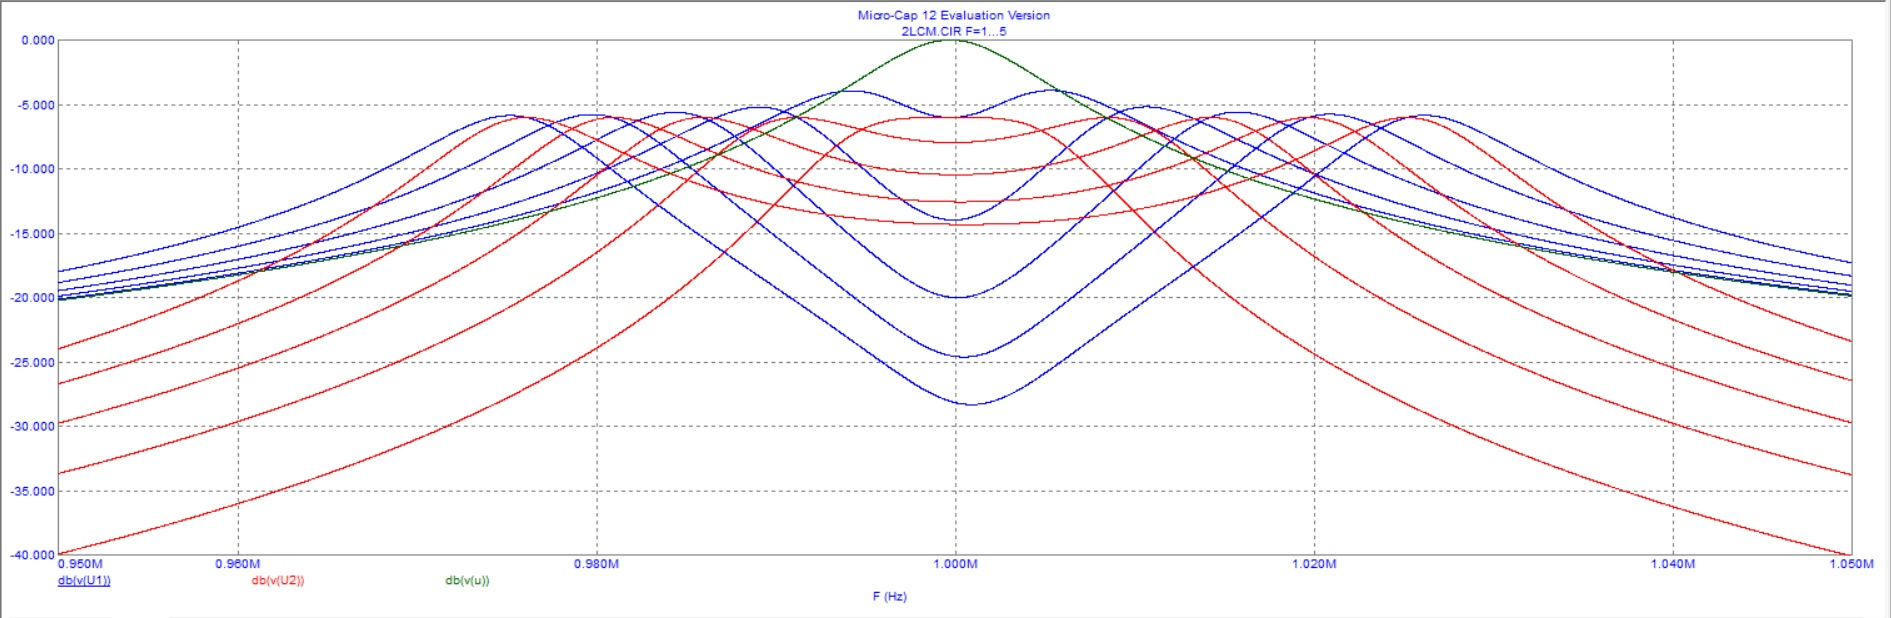
\includegraphics[width=1.1\linewidth]{1.7varF.jpg}
            \caption{варьирование $F [1, 5 \: | \: 1]$}
	\label{A}1
\end{figure}


\begin{figure}[h!]
	\centering
			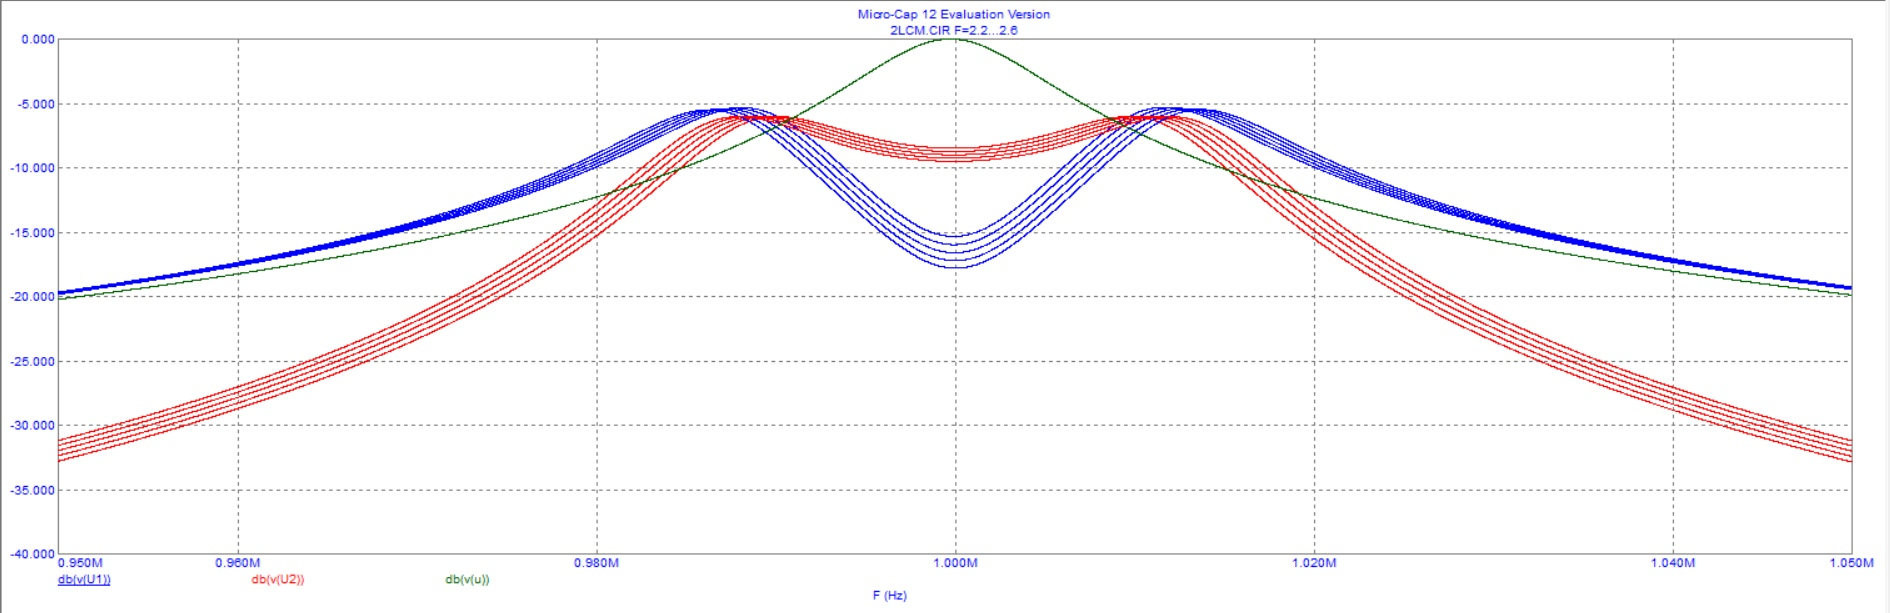
\includegraphics[width=1.1\linewidth]{1.7varF2.jpg}
            \caption{варьирование $F [2.2, 2.6 \: | \: 0.1]$}
	\label{A}
\end{figure}



\subsection{затухания в контуре}
При критической связи $F = 1$ измерим затухания на втором контуре при расстройках на декаду $f_0$. Изучим зависимость уровней затухания от $F = [1,5.5|1.5]$.


\begin{table}[]
	\label{t2}
	\begin{tabular}{|c|c|c|}
	\hline 
		& \multicolumn{2}{c|}{\begin{tabular}[c]{@{}c@{}}Уровень затухания,\\ $\frac{dB}{\text{дек}}$\end{tabular}} \\ \hline
		$F$   & \multicolumn{1}{c|}{f = $100k$}                              & f = $10Meg$                              \\ \hline
		$1$   & \multicolumn{1}{c|}{$-94$}                                   & $-133$                                   \\ \hline
		$2.5$ & \multicolumn{1}{c|}{$-85$}                                   & $-126$                                   \\ \hline
		$4$   & \multicolumn{1}{c|}{$-82$}                                   & $-122$                                   \\ \hline
		$5.5$ & \multicolumn{1}{c|}{$-79$}                                   & $-119$                    \\ \hline       
	\end{tabular}
	\caption{Зависимость уровней затухания от $F$}.
\end{table} 


\begin{figure}[h!]
	\centering
			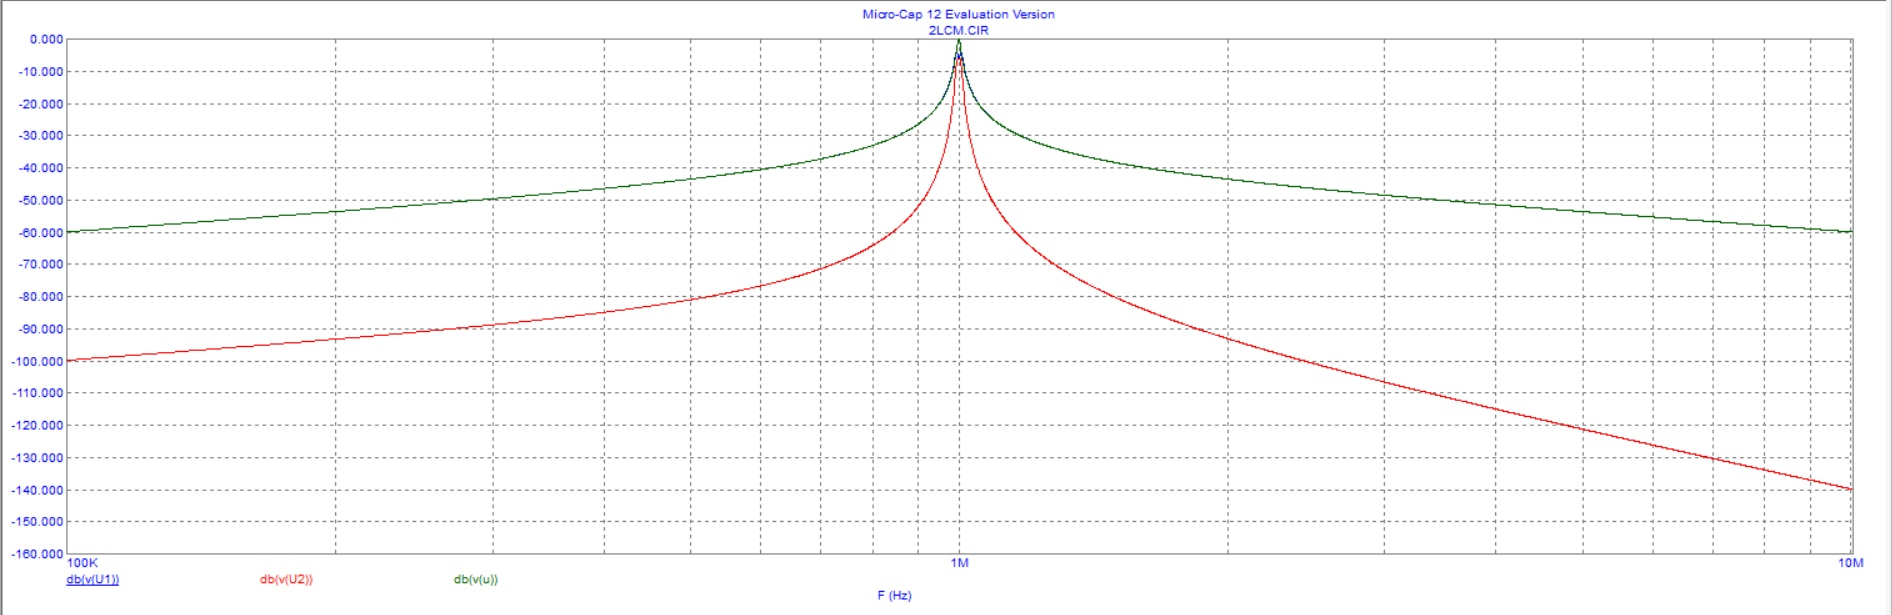
\includegraphics[width=1.1\linewidth]{1.8.jpg}
            %\caption{Задание 1,  пункт 8}
	\label{A}
\end{figure}

\begin{figure}[h!]
	\centering
			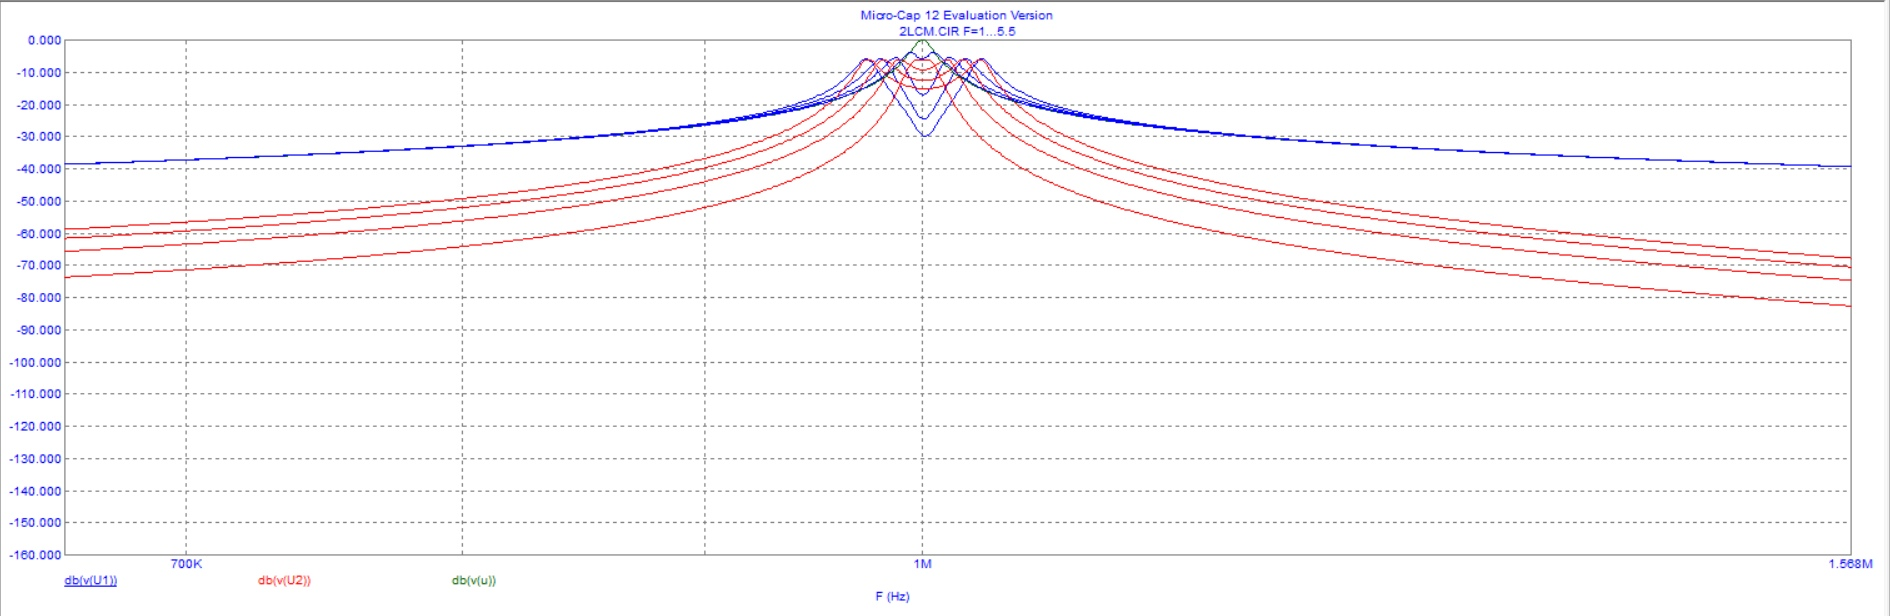
\includegraphics[width=1.1\linewidth]{1.8_VarF.jpg}
            \caption{варьирование $F [1, 5.5|1.5]$}
	\label{A}
\end{figure}
\newpage
\begin{figure}[h!]
	\centering
			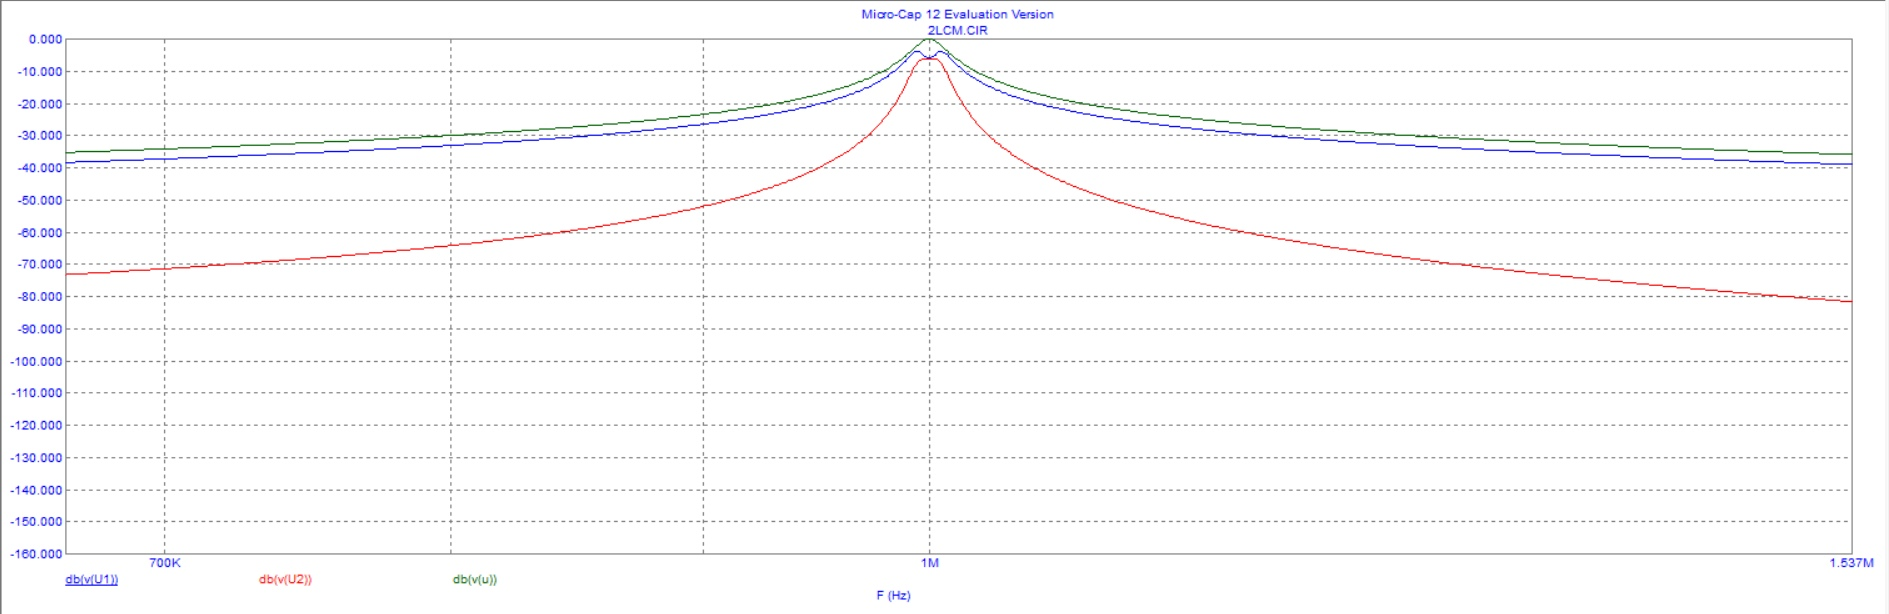
\includegraphics[width=1.1\linewidth]{1.8_VarR.jpg}
            \caption{варьирование $R = [70k, 70k|1k]$}
	\label{A}
\end{figure}

\subsection{плоты 2,4 (ЧХ и графики вносимых проводимостей)}

Снимаем зависимость пиковых значений вещественной и мнимой частей вносимой проводимости при двух различных варьированиях.
\newline
Проверяем формулу $Re(Y) = \frac{F^{2}}{Q\rho}$.

\begin{figure}[h!]
	\centering
			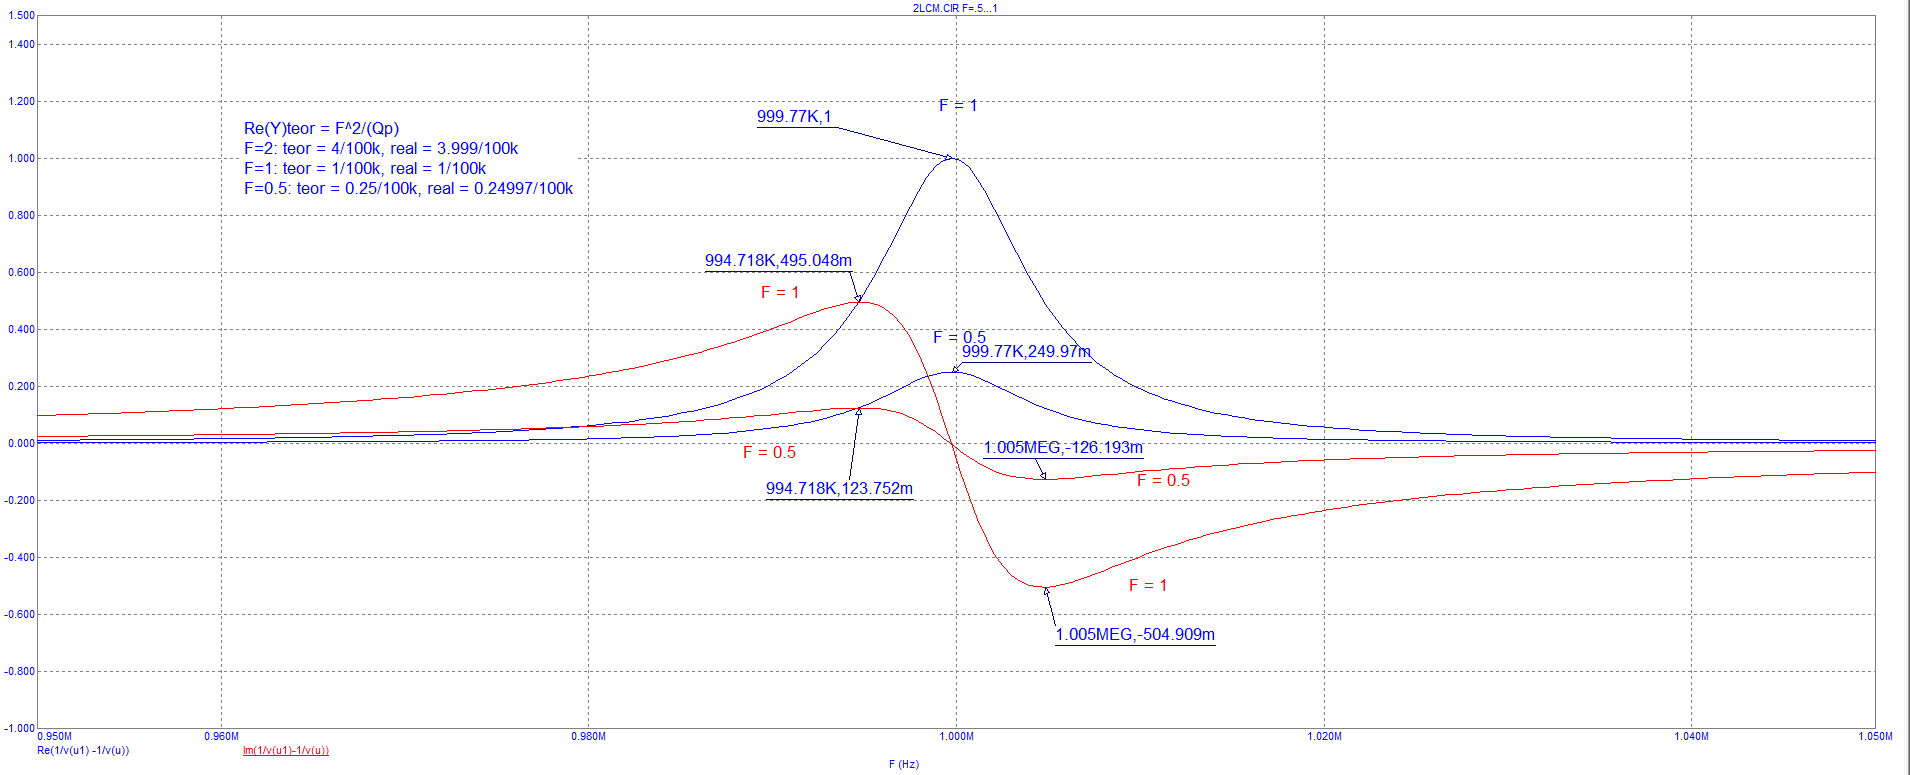
\includegraphics[width=1.1\linewidth]{908_work/9_1.png}
            \caption{варьирование $F [0.5, 1|0.5]$}
	\label{A}
\end{figure}


\begin{figure}[h!]
	\centering
			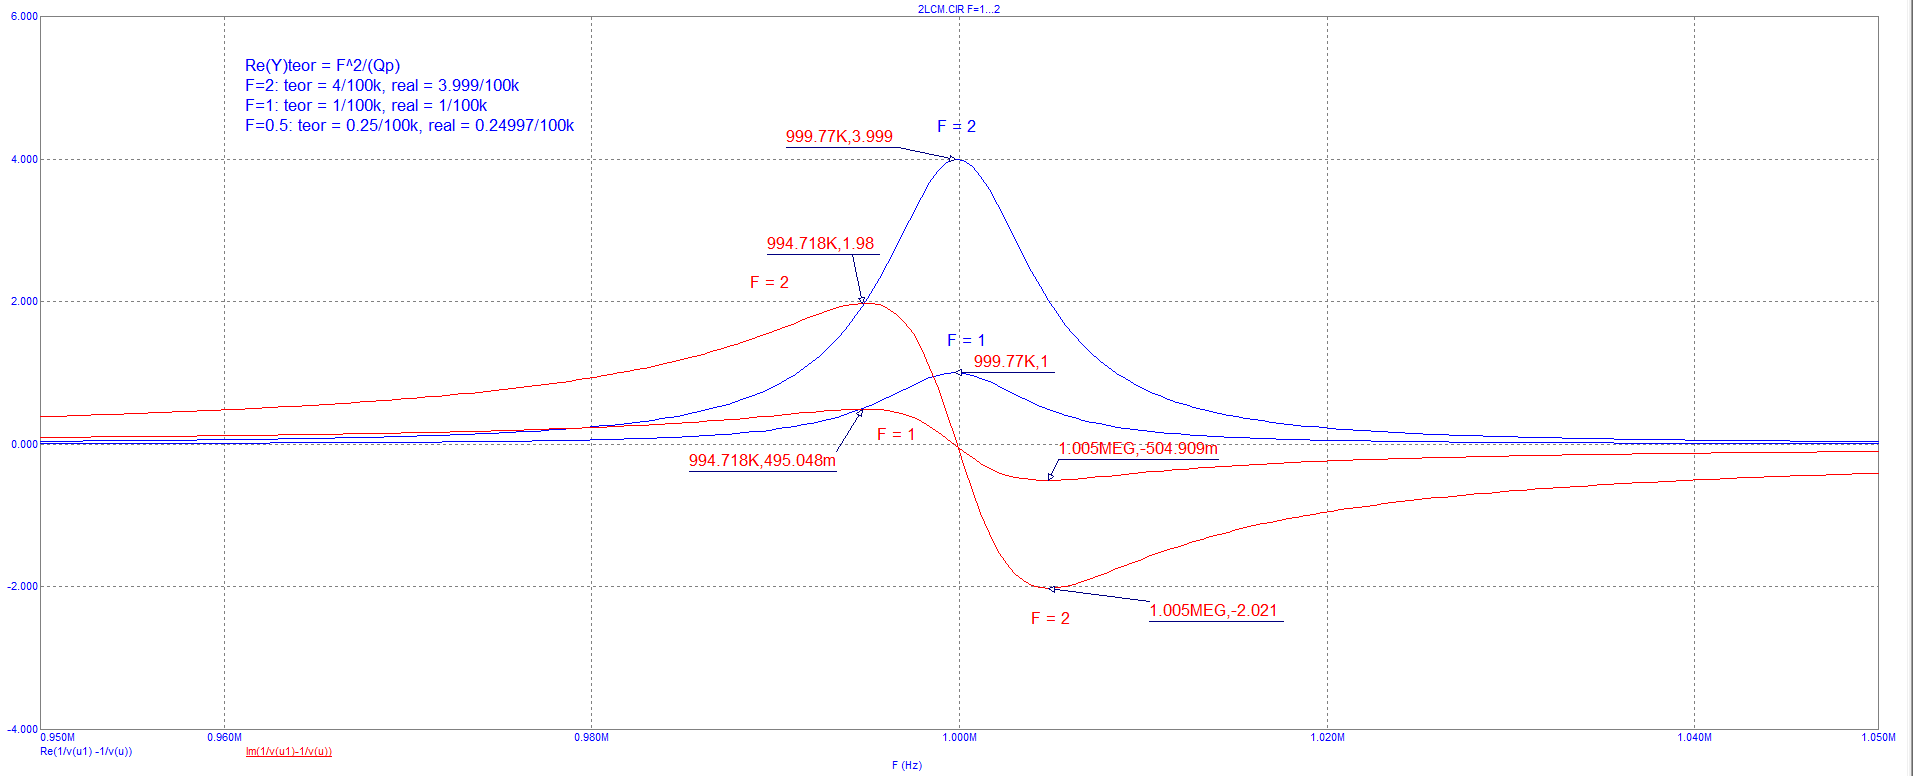
\includegraphics[width=1.1\linewidth]{908_work/9_2.png}
            \caption{варьирование $F [1, 2|1]$}
	\label{A}
\end{figure}


\subsection{переходные характеристики на контурах}

В режиме Transient проанализировать пеереходные характеристики до напряжений на первом и втором контурах при $ F  = 1$. 


\begin{figure}[h!]
	\centering
			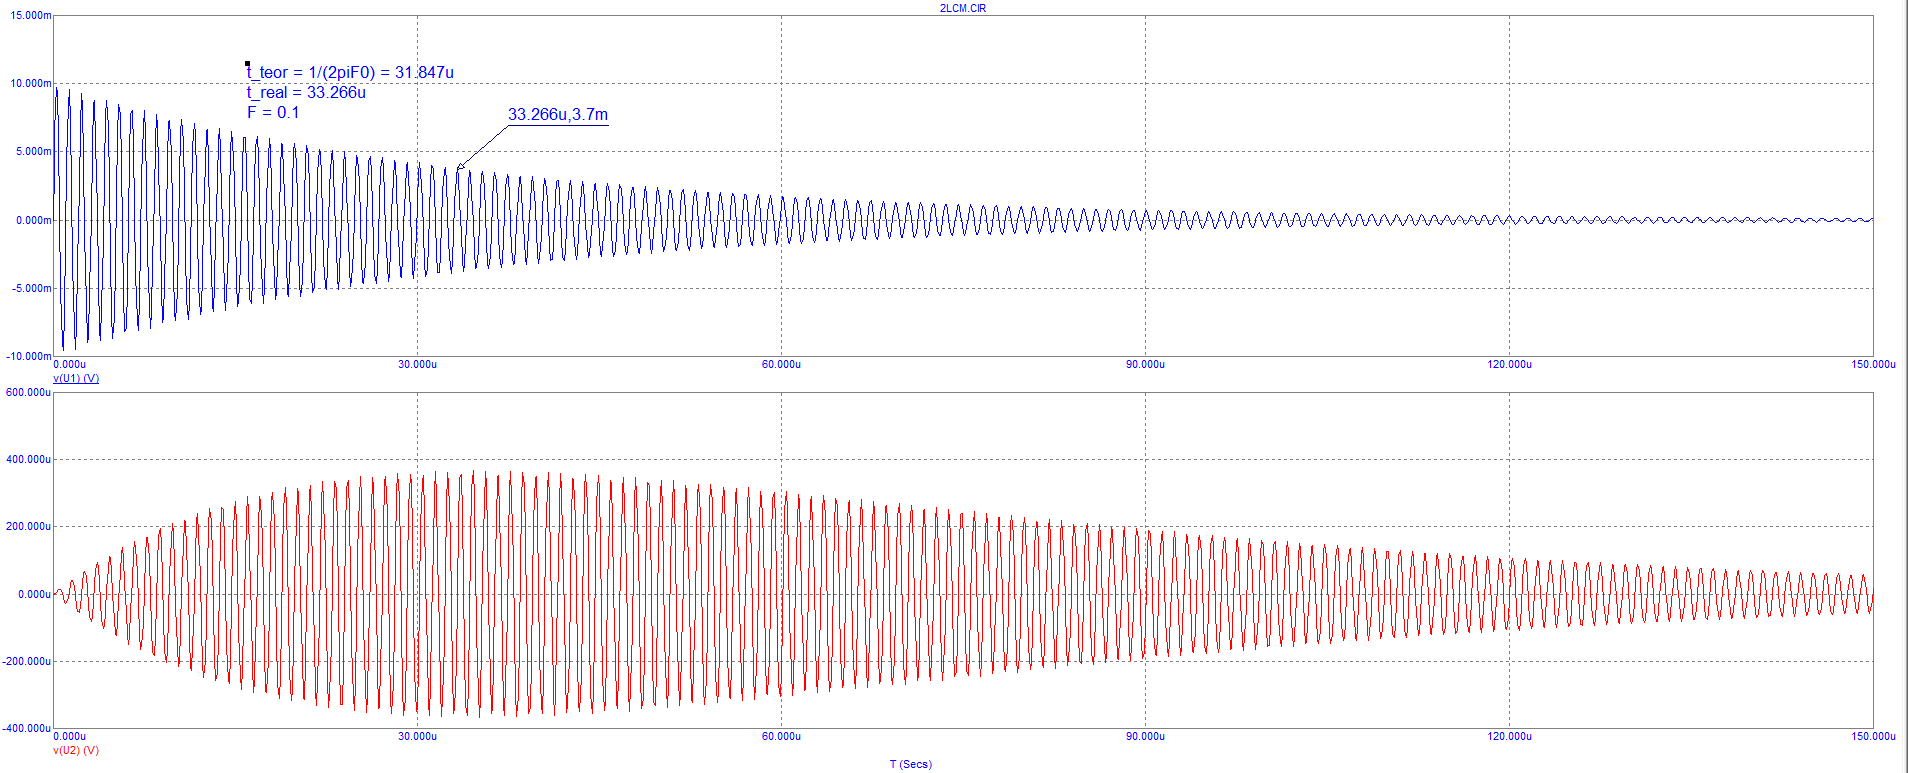
\includegraphics[width=1.1\linewidth]{908_work/10_2.png}
            \caption{$F = 1$}
	\label{A}
\end{figure}

Варьируем $F [0.1, 0.1|1]$. 

\begin{figure}[h!]
	\centering
			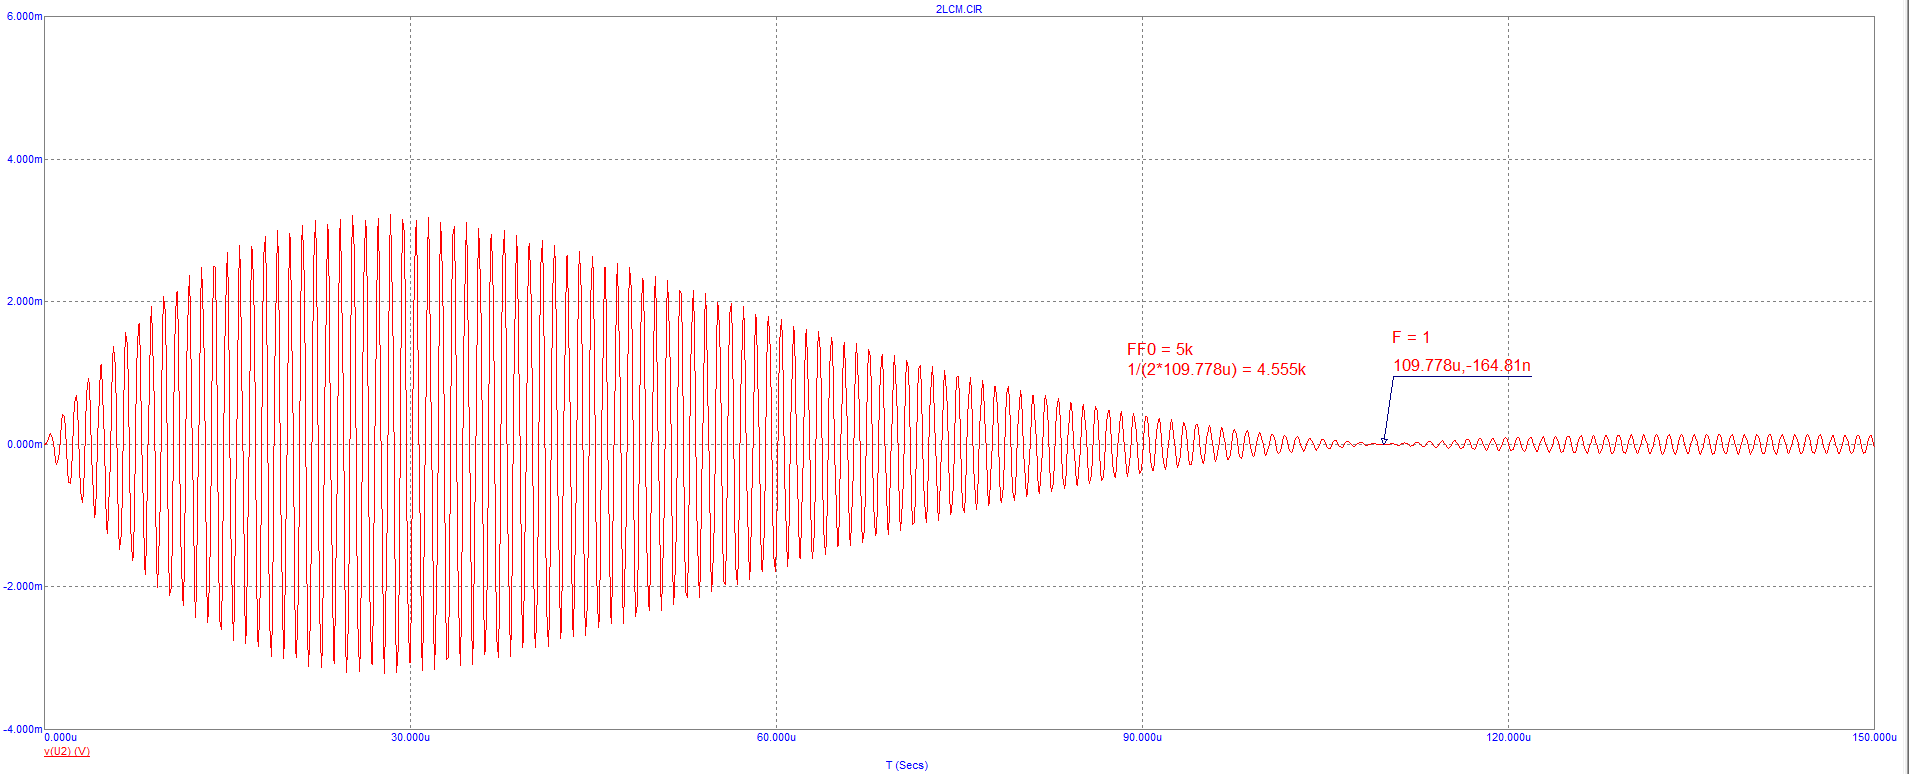
\includegraphics[width=1.1\linewidth]{908_work/10_3_f1.png}
            \caption{варьирование $F [0.1, 0.1|1]$}
	\label{A}
\end{figure}


Варьируем $F [2, 2|1]$

\begin{figure}[h!]
	\centering
			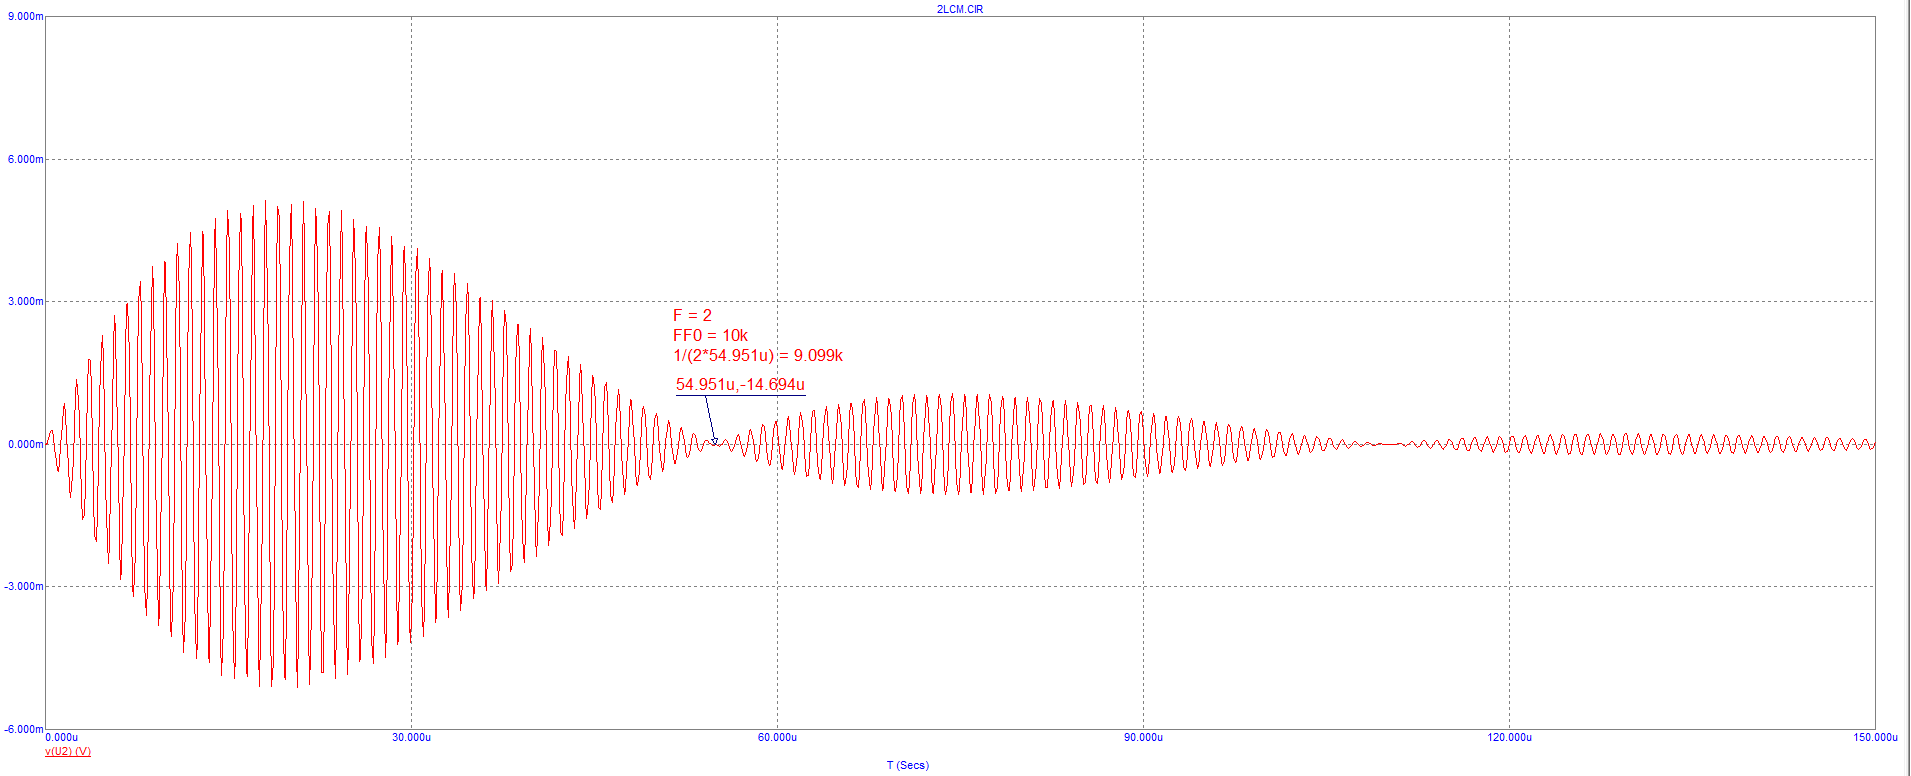
\includegraphics[width=1.1\linewidth]{908_work/10_3_f2.png}
            \caption{варьирование $F [2, 2|1]$}
	\label{A}
\end{figure}

Варьируем  $F  [4, 4|1]$

\begin{figure}[h!]
	\centering
			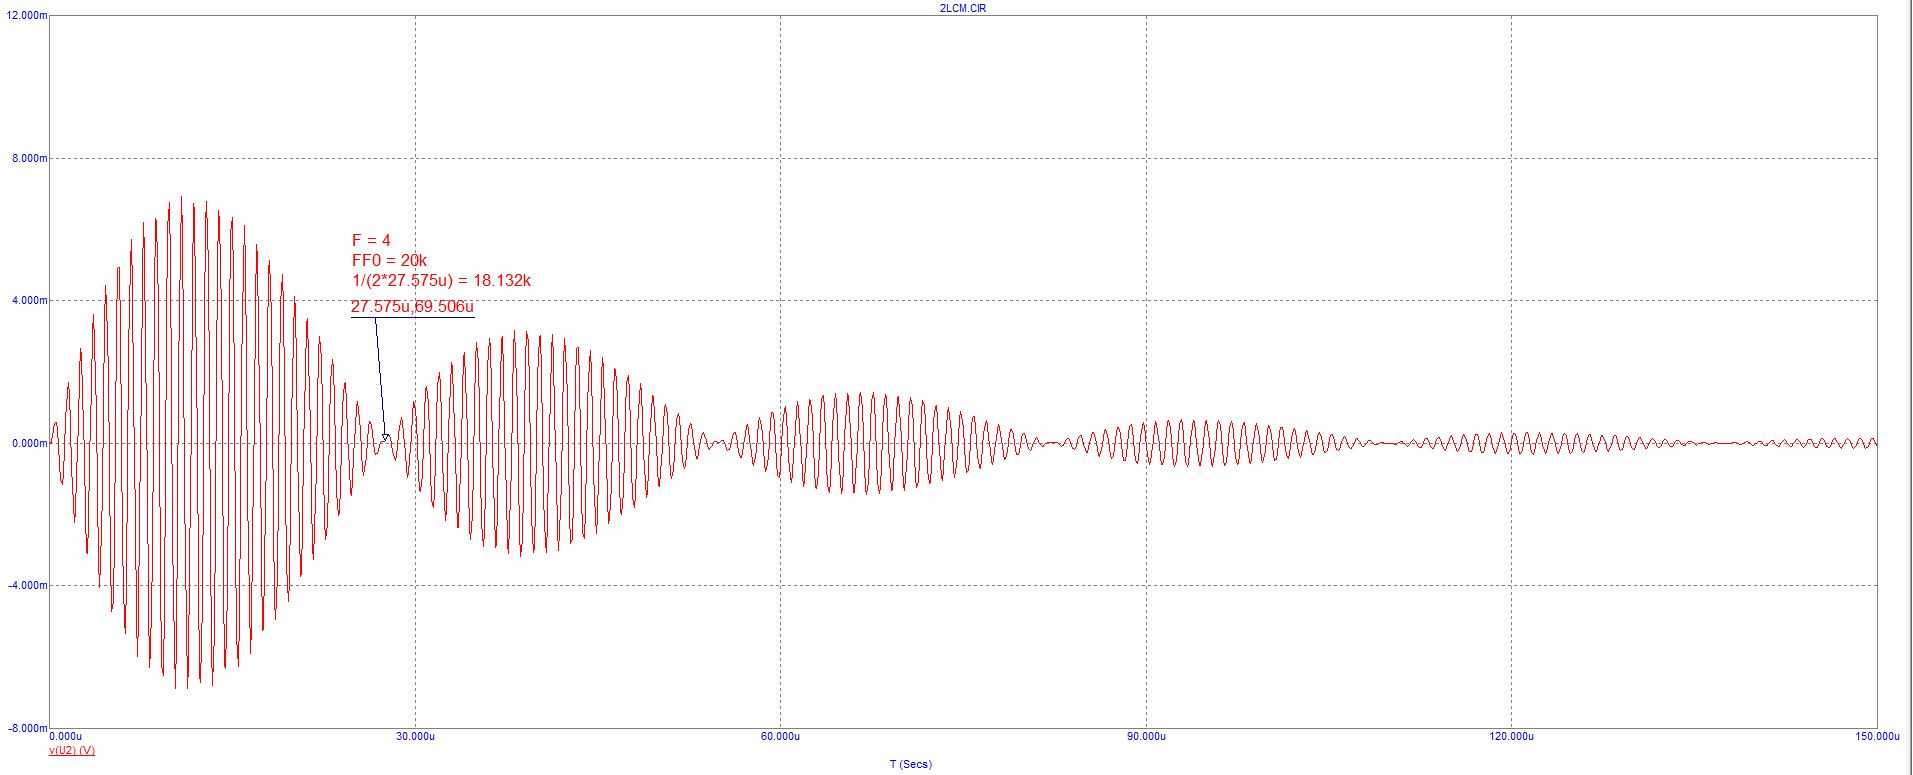
\includegraphics[width=1.1\linewidth]{908_work/10_3_f4.png}
            \caption{варьирование $F  [4, 4|1]$}
	\label{A}
\end{figure}

Варьируем $F [8, 8|1]$

\begin{figure}[h!]
	\centering
			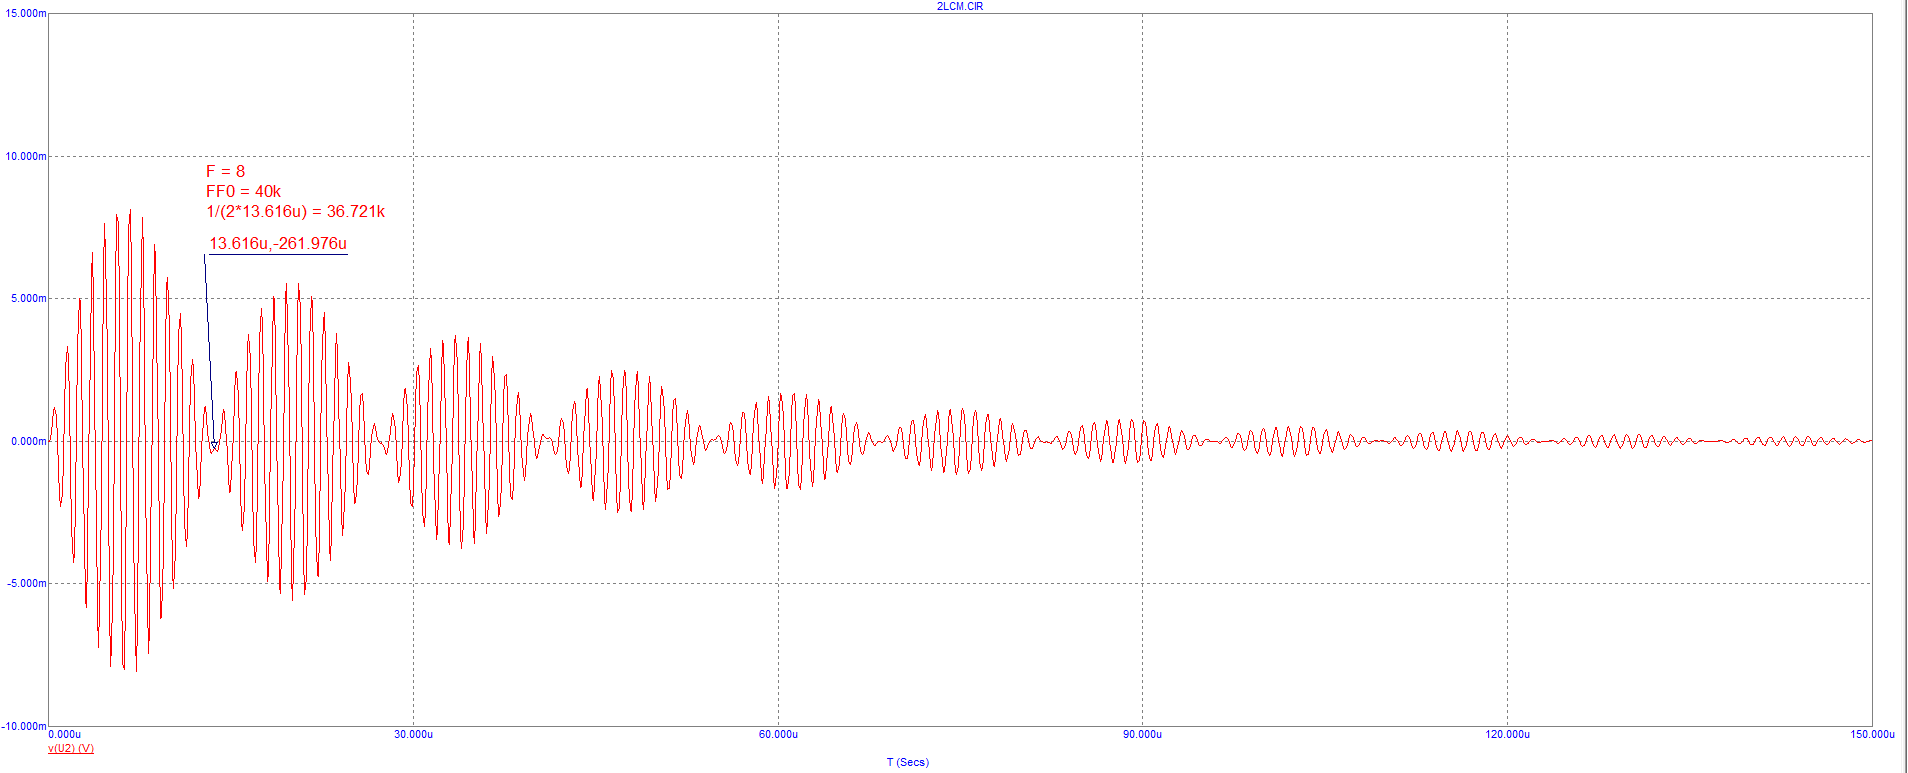
\includegraphics[width=1.1\linewidth]{908_work/10_3_f8.png}
            \caption{варьирование $F [8, 8|1]$}
	\label{A}
\end{figure}

Все расчеты, проверки приведны на скриншотах в данном пункте.

\subsection{ФЧХ при сильной связи}

Установив диапазон моделирования $[2Meg, 600k]$, исследуем частотные и фазовые характеристики при сильной связи. 
\newline
Измерим частоты $f_{\pm}$ пиков при $F = 50$: $f_{+} = 1.414M$, $f_{-} = 816.23k$.
\newline
Проверяем формулу: $f_{\pm} = \frac{f_0}{\sqrt{1 \pm k}}$

\begin{figure}[h!]
	\centering
			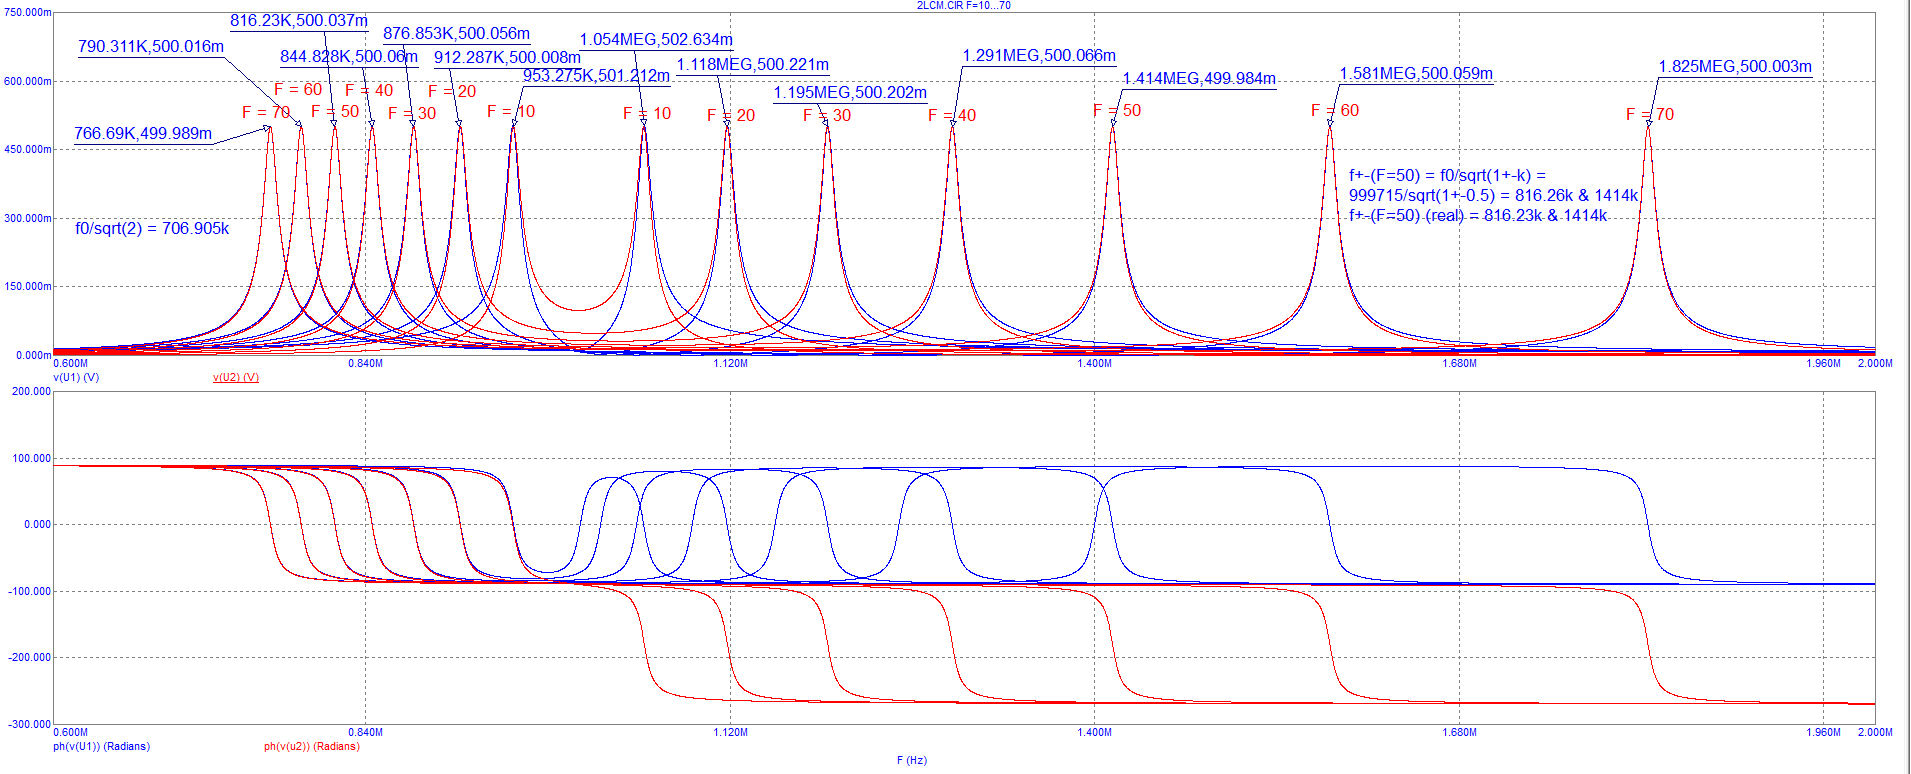
\includegraphics[width=1.1\linewidth]{908_work/11_1.png}
            \caption{варьирование $F  [10, 70|10]$}
	\label{A}
\end{figure}


\begin{figure}[h!]
	\centering
			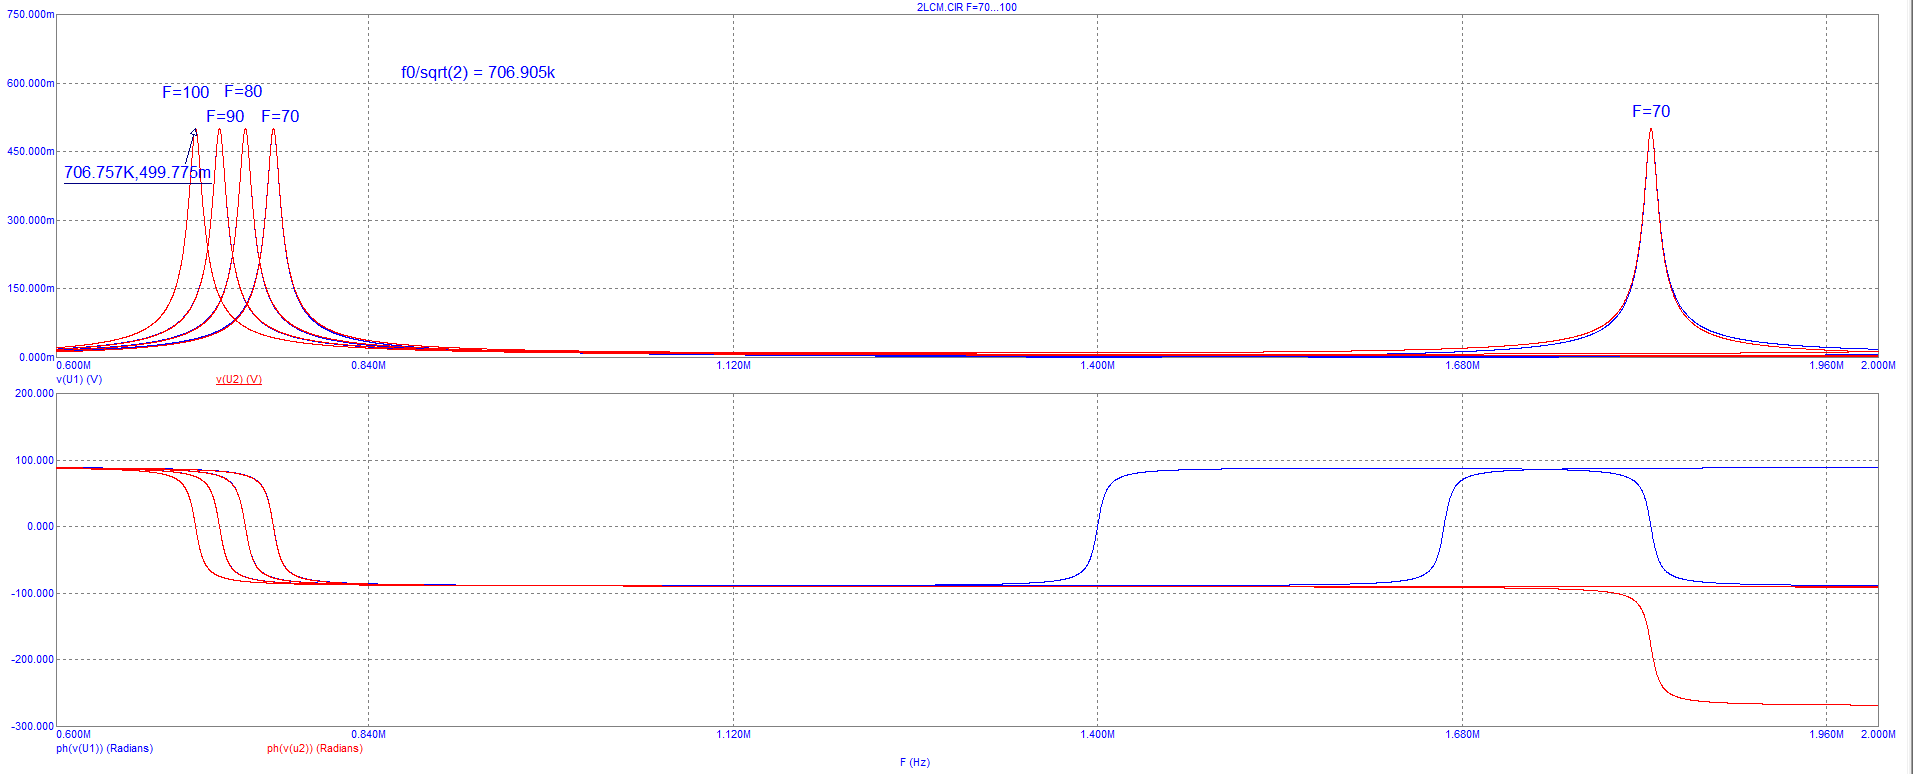
\includegraphics[width=1.1\linewidth]{908_work/11_2.png}
            %\caption{Задание 1,  пункт 11}
	\label{A}
\end{figure}

\newpage

\section{Задание №2. Система с ёмкостной связью.}

\subsection{ФЧХ}

Измерим диапазоны изменения фазовых характеристик на первом и втором контурах:

\begin{figure}[h!]
	\centering
			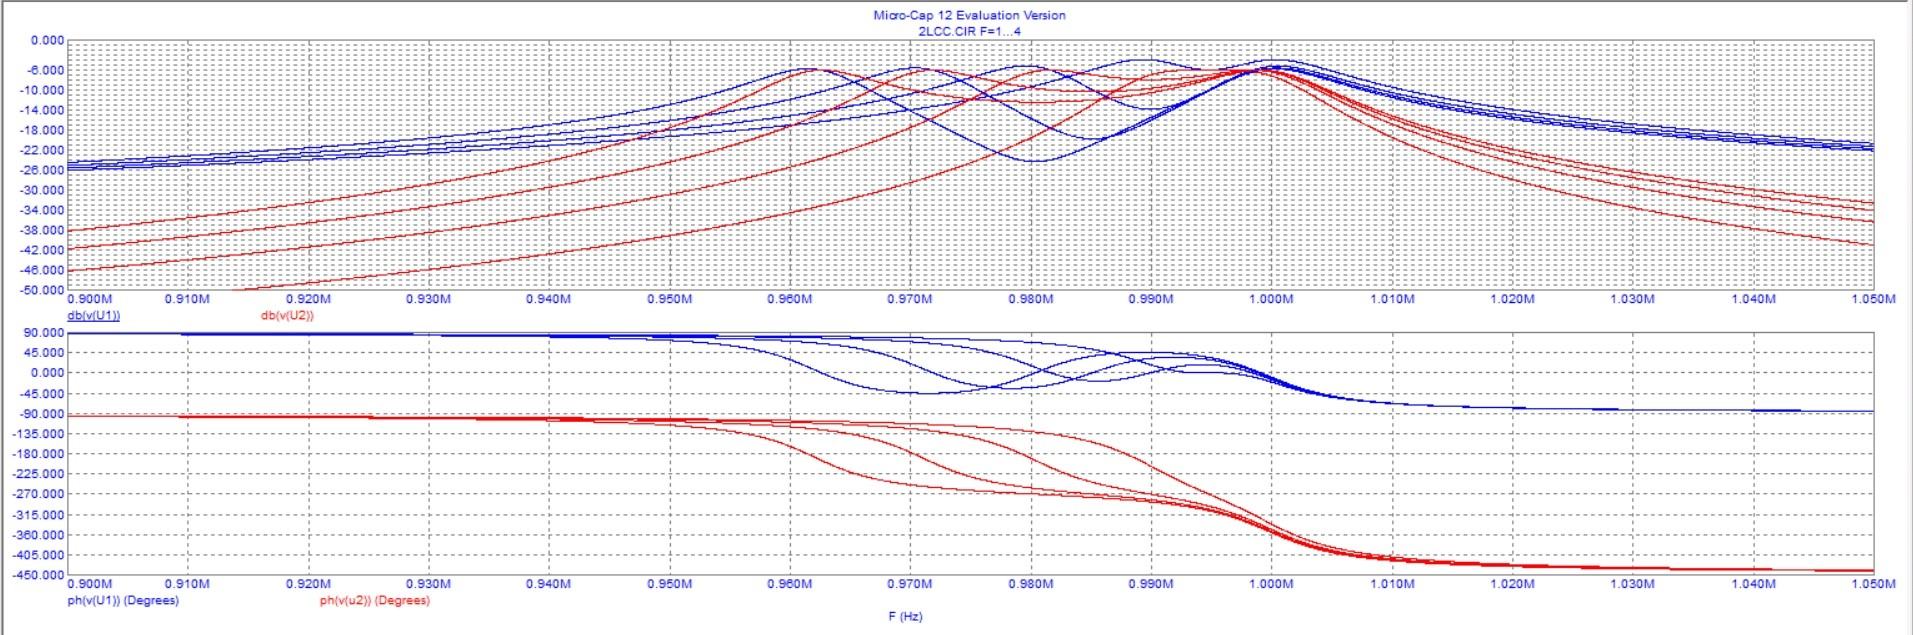
\includegraphics[width=1.1\linewidth]{2.1_varF1.jpg}
            \caption{варьирование $F  [1, 4|1]$}
	\label{A}
\end{figure}


на 1 контуре -- от $90^{\circ}$ до $-90^{\circ}$

на 2 контуре -- от $-90^{\circ}$ до $-450^{\circ}$.

Измерим значения $F$, при которых возникает:
\newline
a) провал на первом контуре ($F = 0.5$).
\newline
b) провал на втором контуре ($F = 1$) c) подъём на фазовой характеристике первого контура ($F = 1$).

Снимем зависимость частоты провала на втором контуре от $F = [2, 4|1]$.

\begin{figure}[h!]
	\centering
			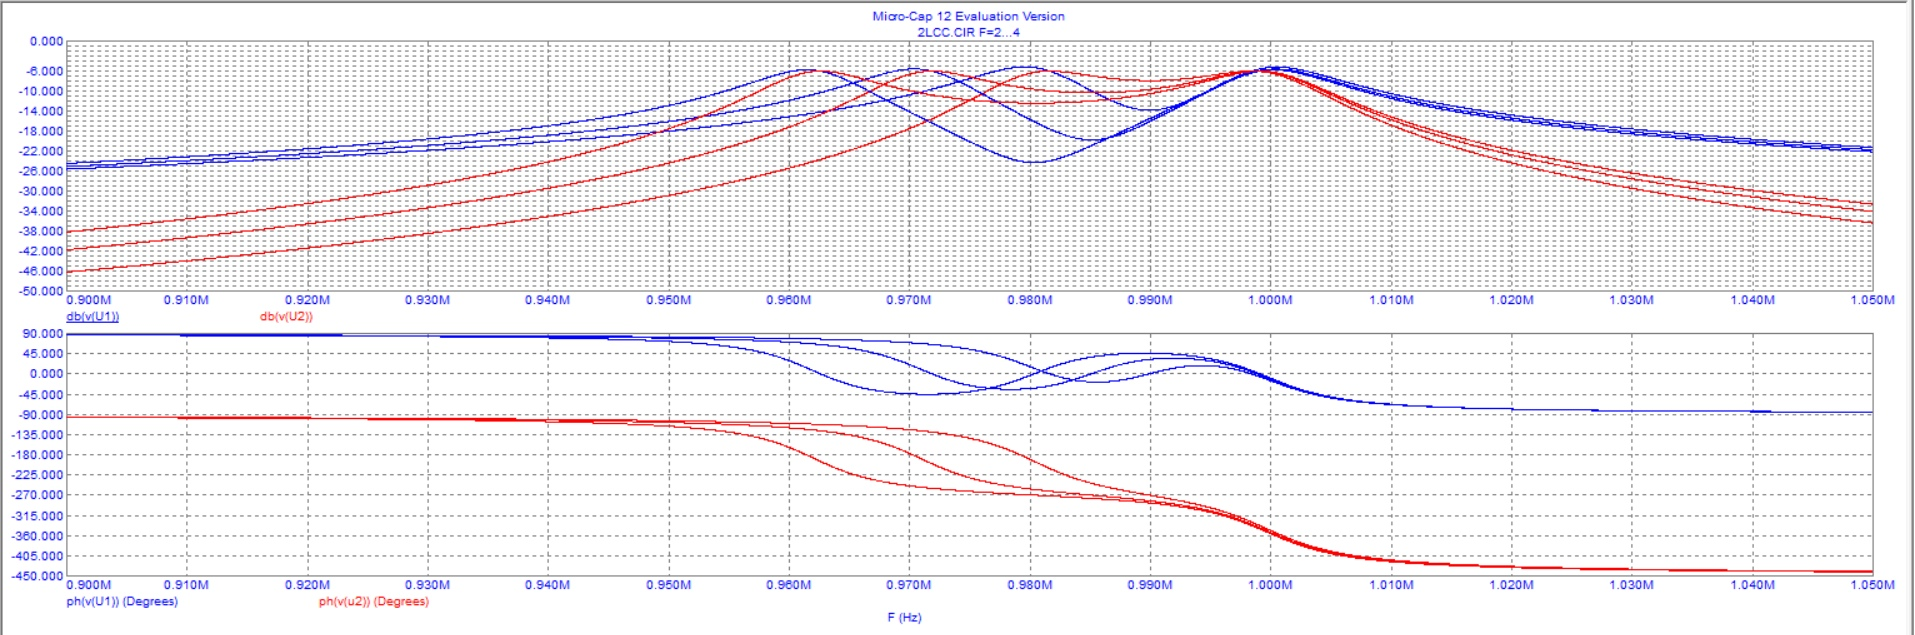
\includegraphics[width=1.1\linewidth]{2.1_varF2.jpg}
            \caption{варьирование $F  [2, 4|1]$}
	\label{A}
\end{figure}


\begin{table}[h!]
	\label{t3}
	\begin{tabular}{|c|c|c|c|}
		\hline 
		$F$               & $2$    & $3$    & $4$    \\ \hline
		$f_{\text{пров}},~\text{Гц}$ & $990k$ & $985k$ & $980k$ \\ \hline
	\end{tabular}
		\caption{Зависимость частоты провала от $F$. }

\end{table}

~

\subsection{исследование изменений ЧХ}

Измерим уровни затухания при расстройках на $\pm 50k$:

\begin{figure}[h!]
	\centering
			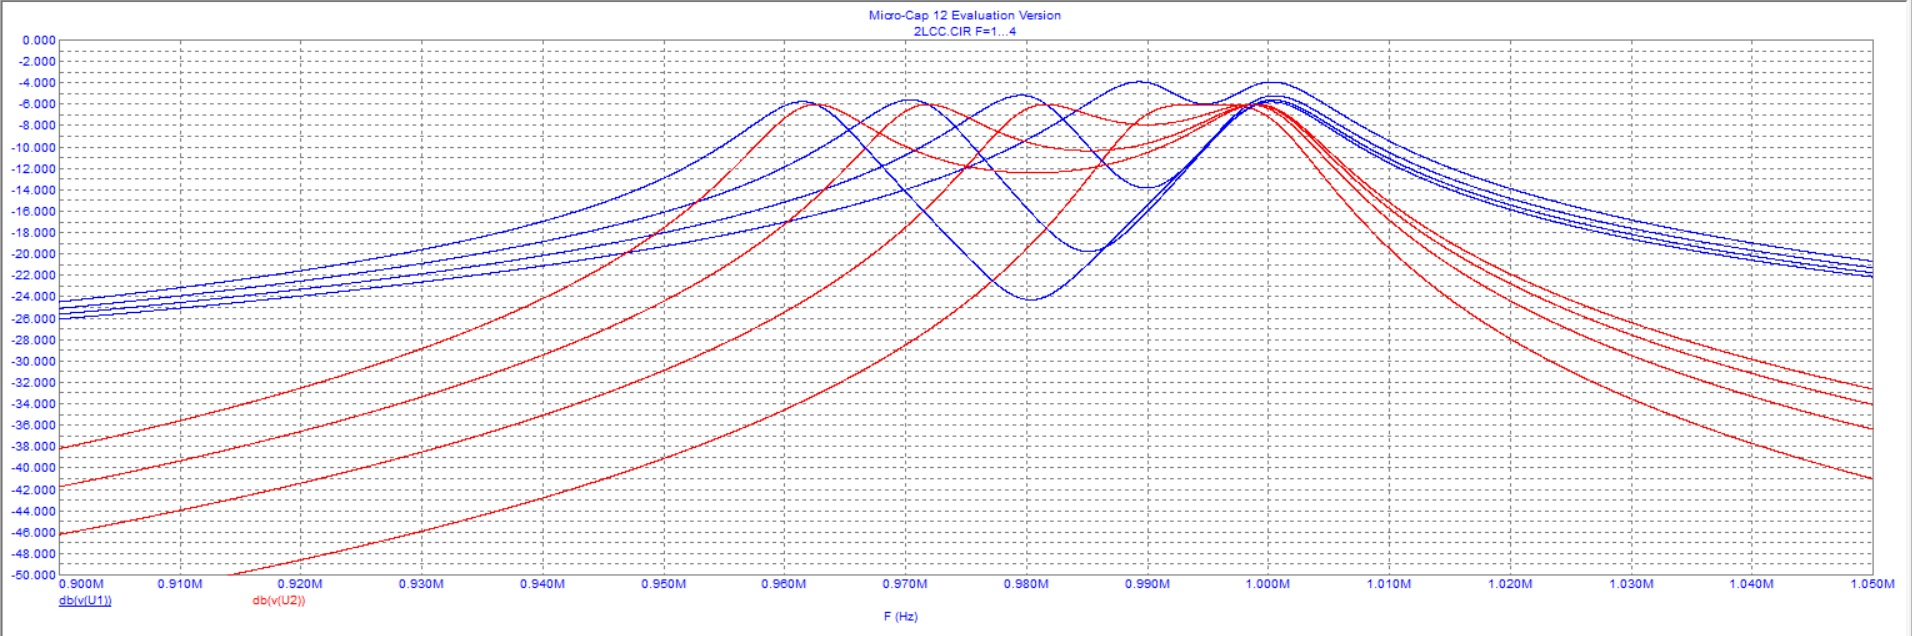
\includegraphics[width=1.1\linewidth]{2.2_varF.jpg}
            \caption{варьирование $F  [1,4|1]$}
	\label{A}
\end{figure}

1 контур -- $-17 \frac{dB}{\text{дек}}$

2 контур -- $-35 \frac{dB}{\text{дек}}$.

Перейдём на частотный диапазон $[10Meg,100k]$ и измерим уровни затухания при расстройках на декаду $f_0$:

\begin{figure}[h!]
	\centering
			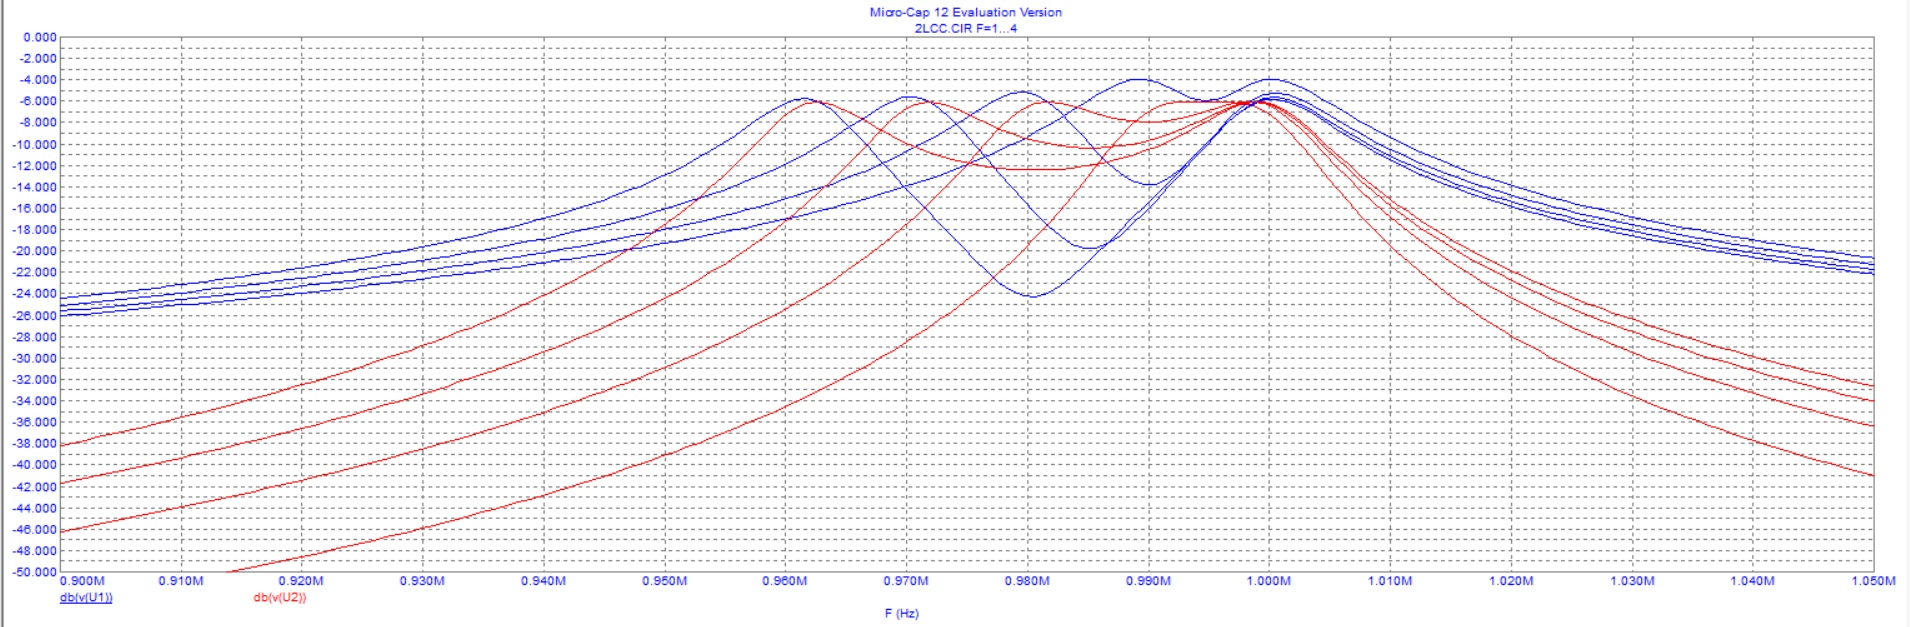
\includegraphics[width=1.1\linewidth]{2.2_freq_range.jpg}
            \caption{частотный диапазон $[10Meg, 100k]$}
	\label{A}
\end{figure}

1 контур -- $-56\frac{dB}{\text{дек}}$

2 контур -- $-94\frac{dB}{\text{дек}}(\text{вблизи $100k$})$, $-133\frac{dB}{\text{дек}}(\text{вблизи $10Meg$})$



\subsection{изучение переходных характеристик при различных $F$}

Изучим  переходные ххарактеристики при значениях $F = 0.1$,  $F = 1$,  $F = 2$,   $F = 4$. Убедимся в их сходстве с характеристиками системы с индуктивной связью. 

\begin{figure}[h!]
	\centering
			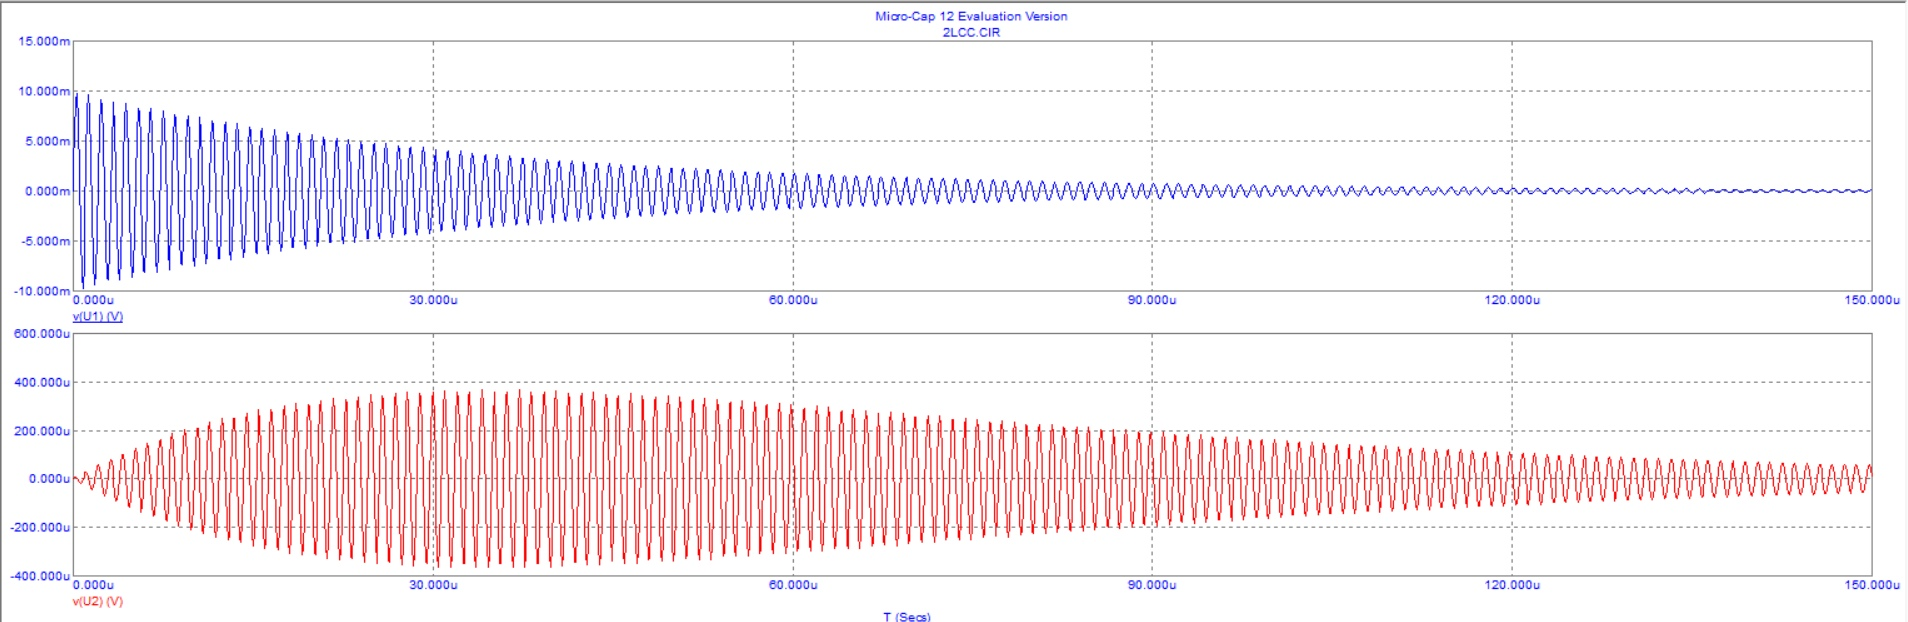
\includegraphics[width=1.1\linewidth]{2.3_varF1.jpg}
            \caption{варьирование $F  [0.1, 0.1|1]$}
	\label{A}
\end{figure}

\newpage

$ $

\begin{figure}[h]
	\centering
			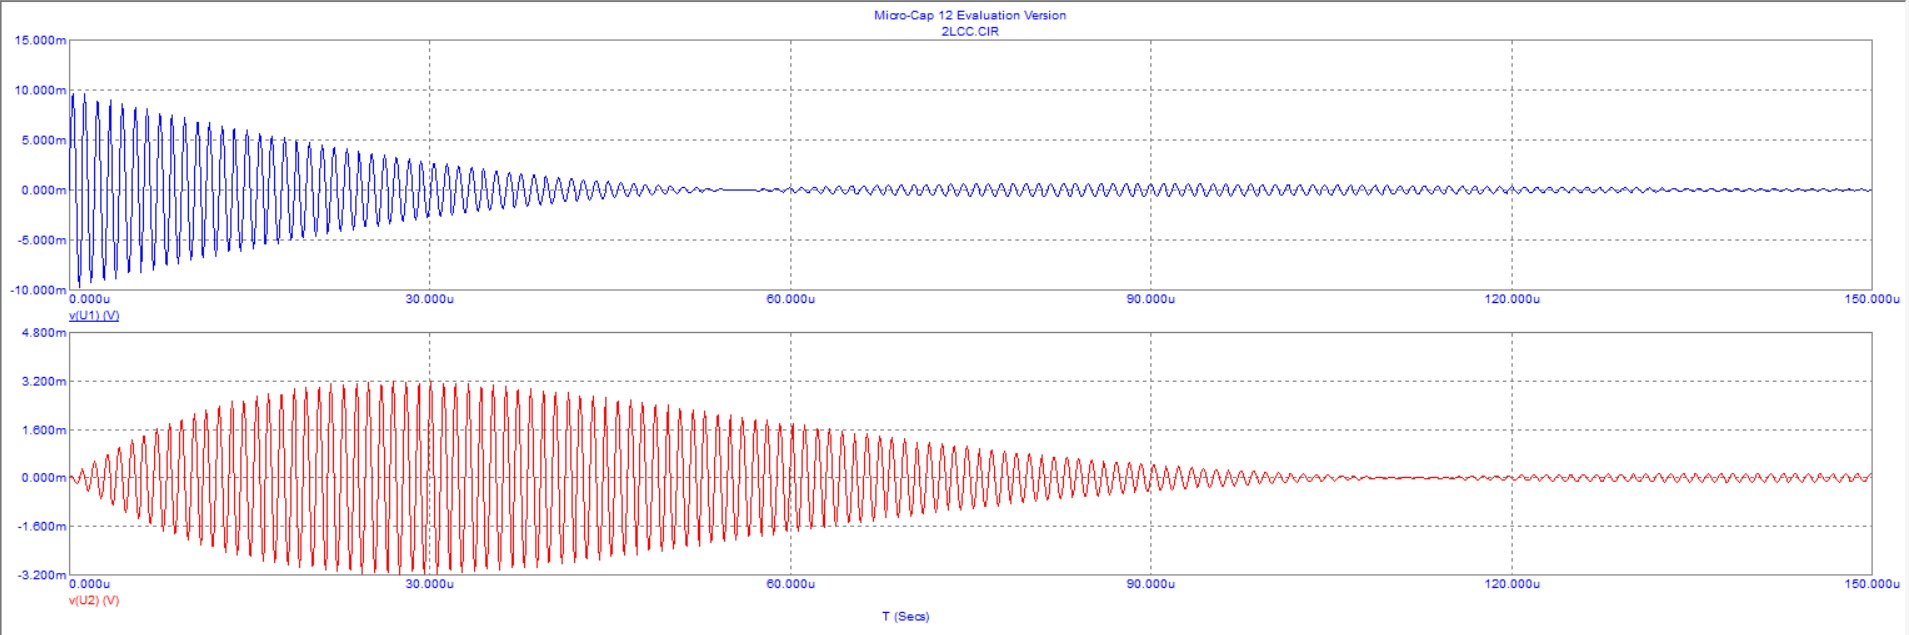
\includegraphics[width=1.1\linewidth]{2.3_varF2.jpg}
            \caption{варьирование $F  [1, 1|1]$}
	\label{A}
\end{figure}

\begin{figure}[h]
	\centering
			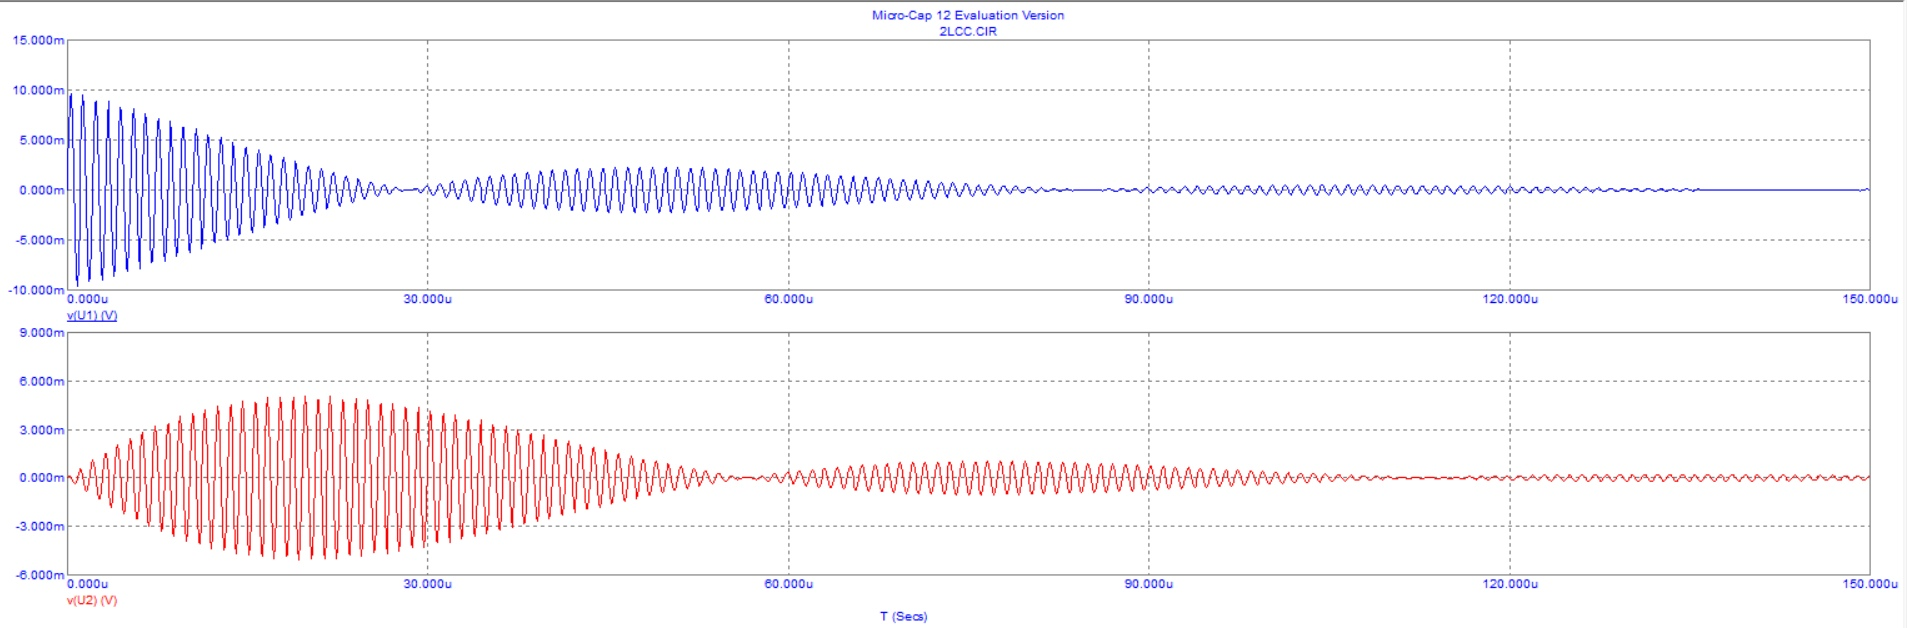
\includegraphics[width=1.1\linewidth]{2.3_varF3.jpg}
            \caption{варьирование $F   [2, 2|1]$}
	\label{A}
\end{figure}

\begin{figure}[h]
	\centering
			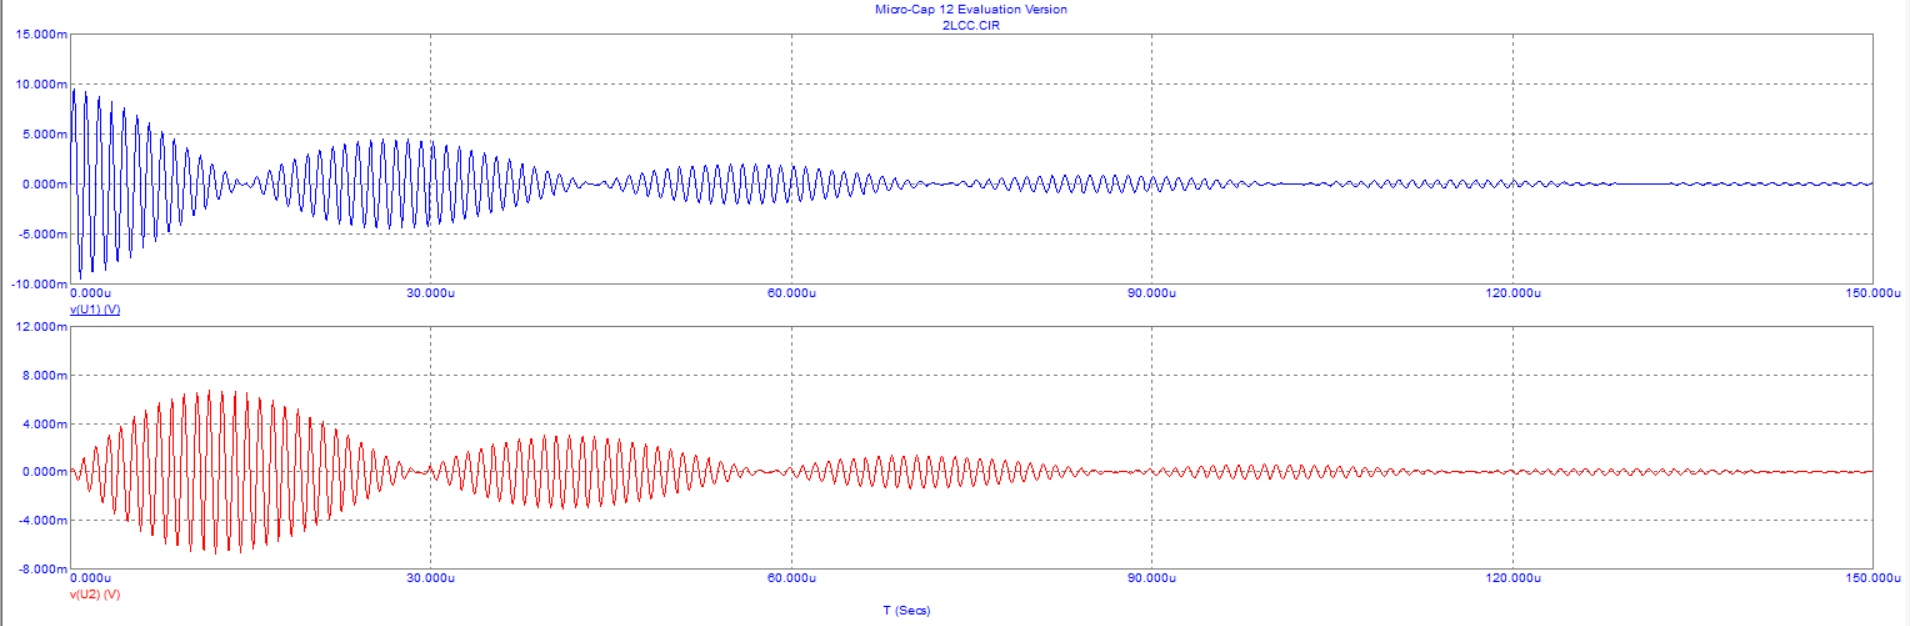
\includegraphics[width=1.1\linewidth]{2.3_varF4.jpg}
            \caption{варьирование $F  [4, 4|1]$}
	\label{A}
\end{figure}

\newpage

\section{Литература}

\begin{itemize}

\item Григорьев А.А. Лекции по теории связанных колебательных контуров. - М.: МФТИ, $2013 .$

\item Методические указания к работе №$20 (\text{Свзяанные колебательные контуры})$.

\end{itemize}

\end{document}